\subsection{导子的泛问题；交换情形}

现在假设 A 是一个交换 K-代数，E 是一个 A-模；可以把 E 看作一个 (A, A)-双模，其两个外合成律都与给定的 A-模运算相同。另一方面，\(A \otimes_{K} A\) 上的 (A, A)-双模结构与其 \((A \otimes_{K} A)\) -模结构相同，后者源自 \(A \otimes_{K} A\) 上的交换环结构，因为在这种情形下，对于 A 中的 x、y、u、v，

\[
x. (u \otimes v). y = (x u) \otimes (v y) = (x u) \otimes (y v) = (x \otimes y) (u \otimes v).
\]

因此在这种情形下，\(\mathfrak{J}\) 作为 \(m\) 的核是环 \(\mathbf{A} \otimes_{\mathbb{K}} \mathbf{A}\) 的理想，并且，由于 \(m: \mathbf{A} \otimes_{\mathbb{K}} \mathbf{A} \to \mathbf{A}\) 是满射的， \((\mathbf{A} \otimes_{\mathbb{K}} \mathbf{A}) / \mathfrak{J}\) 同构于 \(\mathbf{A}\) ；若还把 \(\mathbf{E}\) 视为一个 \((\mathbf{A} \otimes_{\mathbb{K}} \mathbf{A})\) -模，即经由 \(m\) （换言之，即 \((\mathbf{A} \otimes_{\mathbb{K}} \mathbf{A})\) -模 \(m_*(\mathbf{E})\) ），则 \((\mathbf{A}, \mathbf{A})\) -双模同态 \(\mathfrak{J} \to \mathbf{E}\) 便与 \((\mathbf{A} \otimes_{\mathbb{K}} \mathbf{A})\) -模同态 \(\mathfrak{J} \to \mathbf{E}\) 相等同 ( \(\S 4, no. 3\) )，换言之，存在一个典范的 \(\mathbf{K}\) -模同构

\[
\operatorname{Hom} _ {(\mathbf {A}, \mathbf {A})} (\mathfrak{J} , \mathrm{E}) \rightarrow \operatorname{Hom} _ {\mathbf {A} \otimes_ {\mathbf {K}} \mathbf {A}} (\mathfrak{J} , \mathrm{E}).
\]

另一方面， \(\mathfrak{J}\mathbf{E} = \{0\}\) ，因为元素 \(1 \otimes x - x \otimes 1\) 生成 \(\mathfrak{J}\) （作为 \((\mathbf{A} \otimes_{\mathbb{K}} \mathbf{A})\) -模；第10号，引理1），并且对所有 \(z \in \mathbf{E}\) ，

\[
(1 \otimes x - x \otimes 1) z = 0
\]

这是根据 E 上 \((\mathbf{A} \otimes_{\mathbf{K}} \mathbf{A})\) -模结构的定义。由于 \(\mathfrak{J}\) 包含在 \((\mathbf{A} \otimes_{\mathbf{K}} \mathbf{A})\) -模 E 的零化子中，且 \(((\mathbf{A} \otimes_{\mathbf{K}} \mathbf{A})/\mathfrak{J})\) -模 E 上的模结构按定义正是最初给定的 E 上的 A-模结构，因此，考虑到

\[
\mathfrak{J} \otimes_ {\mathbf {K}} ((\mathbf {A} \otimes_ {\mathbf {K}} \mathbf {A}) / \mathfrak{J})
\]

到 \(\mathfrak{J} / \mathfrak{J}^2\) （§ 4，第 1 号，命题 1 的推论 1）的典范同构，存在一个典范的 K-模同构

\[
\operatorname{Hom} _ {\mathbf {A} \otimes_ {\mathbf {K}} \mathbf {A}} (\mathfrak{J} , \mathrm{E}) \rightarrow \operatorname{Hom} _ {\mathbf {A}} (\mathfrak{J} / \mathfrak{J}^ {2}, \mathrm{E}).
\]

考虑到第10节命题17，可见我们已证明以下命题：

命题18。设 A 是一个交换 K-代数，且 \(\mathfrak{J}\) 是这样一个理想：它是满射典范同态 \(m: \mathbf{A} \otimes_{\mathbf{K}} \mathbf{A} \to \mathbf{A}\) 的核，于是 A 同构于 \((\mathbf{A} \otimes_{\mathbf{K}} \mathbf{A}) / \mathfrak{J}\) ，且 \(\mathfrak{J} / \mathfrak{J}^2\) 典范地具有一个 A-模结构。设 \(d_{\mathbf{A} / \mathbf{K}}: \mathbf{A} \to \mathfrak{J} / \mathfrak{J}^2\) 是使每个 \(x \in \mathbf{A}\) 对应 \(x \otimes 1 - 1 \otimes x\) 模 \(\mathfrak{J}^2\) 的同余类的 K-线性映射。映射 \(d_{\mathbf{A} / \mathbf{K}}\) 是一个 K-导子，并且对于每个 A-模 E 和每个 K-导子 D： \(\mathbf{A} \to \mathbf{E}\) ，存在且仅存在一个 A-线性映射 \(g: \mathfrak{J} / \mathfrak{J}^2 \to \mathbf{E}\) ，使得 \(\mathrm{D} = g \circ d_{\mathbf{A} / \mathbf{K}}\) .

A-模 \(\mathfrak{J} / \mathfrak{J}^2\) 称为 A 的 K-微分模，记作 \(\Omega_{\mathbf{K}}(\mathbf{A})\) ；对所有 \(x \in \mathbf{A}\) ， \(d_{\mathbf{A} / \mathbf{K}}(x)\) （也记作 \(dx\) ）称为 \(x\) 的微分；已经看到（第10号，引理1），元素 \(d_{\mathbf{A} / \mathbf{K}}(x)\) （ \(x \in \mathbf{A}\) ）构成 A-模 \(\Omega_{\mathbf{K}}(\mathbf{A})\) 的一个生成系。命题18表明映射 \(g \mapsto g \circ d_{\mathbf{A} / \mathbf{K}}\) 是一个典范 A-模同构

\[
\phi_ {\mathbf {A}}: \operatorname{Hom} _ {\mathbf {A}} (\Omega_ {\mathbf {K}} (\mathbf {A}), \mathrm{E}) \rightarrow \mathrm{D} _ {\mathbf {K}} (\mathrm{A}, \mathrm{E})
\]

（ \(D_{K}(A, E)\) 上的 A-模结构由第5号命题7定义）。

有序对 \((\Omega_{\mathbf{K}}(\mathbf{A}), d_{\mathbf{A}/\mathbf{K}})\) 因而是下述泛映射问题的解，其中 \(\Sigma\) 是 A-模结构的种类，而 \(\alpha\) -映射是从 A 到 A-模的 K-导子（集合论，IV，§3，第1号）。

例。设 M 是一个 K-模；由第9号命题14可知，对于每个 S(M)-模 E，映射 D ↦ D \textbar{} M 定义了 D\_K(S(M), E) 到 Hom\_K(M, E) 的一个 S(M)-模同构；另一方面，由于 E 是 S(M)-模，Hom\_K(M, E) 典范同构于

\[
\operatorname{Hom} _ {\mathbf {S} (\mathbf {M})} (\mathbf {M} \otimes_ {\mathbf {K}} \mathbf {S} (\mathbf {M}), \mathbf {E}),
\]

M 到 E 的每个 K-同态都能唯一地表示为 \(x \mapsto h(x \otimes 1)\) 的形式，其中

\[
h \in \operatorname{Hom} _ {\mathbf {S} (\mathbf {M})} (\mathbf {M} \otimes_ {\mathbf {K}} \mathbf {S} (\mathbf {M}), \mathbf {E})
\]

(II, § 5, 第 1 号)。设 \(\mathbf{D}_0\) 为 K-导子 \(\mathbb{S}(\mathbf{M}) \to \mathbf{M} \otimes_{\mathbb{K}} \mathbb{S}(\mathbf{M})\) ，它限制在 \(\mathbf{M}\) 上是典范同态 \(x \mapsto x \otimes 1\) ；因此每个 K-导子 \(\mathbf{D}: \mathbb{S}(\mathbf{M}) \to \mathbf{E}\) 都可以唯一地写成 \(h \circ \mathbf{D}_0\) ，其中

\[
h \in \operatorname{Hom} _ {\mathbf {S} (\mathbf {M})} (\mathbf {M} \otimes_ {\mathbf {K}} \mathbf {S} (\mathbf {M}), \mathbf {E}).
\]

由泛映射问题解的唯一性可知，存在唯一的S(M)-模同构

\[
\omega : \mathbf {M} \otimes_ {\mathbf {K}} \mathbf {S} (\mathbf {M}) \rightarrow \Omega_ {\mathbf {K}} (\mathbf {S} (\mathbf {M}))
\]

，使得 \(\mathbf{D}_0\circ \omega = d_{\mathbb{S}(\mathbf{M}) / \mathbb{K}}\) ；换言之，对所有 \(x\in \mathbf{M}\) \(\omega (x\otimes 1) = dx.\) 特别是，如果 \(\mathbf{M}\) 是自由 K-模，带有基 \((e_{\lambda})_{\lambda \in \mathbf{L}},\Omega_{\mathbb{K}}(\mathbb{S}(\mathbf{M}))\) 便是自由 S(M)-模，其基由微分 \(de_{\lambda}\) 的集合构成。特别考虑 \(\mathrm{L} = [1,n]\) 的情形，此时 \(\mathbb{S}(\mathbf{M})\) 与多项式代数 \(\mathbf{K}[\mathbf{X}_1,\dots ,\mathbf{X}_n]\) 等同（§ 6，第 6 号）；对每个多项式 \(\mathrm{P}\in \mathrm{K}[\mathrm{X}_1,\dots ,\mathrm{X}_n]\) ，我们可以唯一地写出

\[
d \mathrm{P} = \sum_ {i = 1} ^ {n} \mathrm{D} _ {i} \mathrm{P}. d \mathrm{X} _ {i}
\]

其中 \(D_{i}P \in K[X_{1}, \ldots, X_{n}]\) ，并且，根据上述内容，映射 \(P \mapsto D_{i}P\) 是 \(K[X_{1}, \ldots, X_{n}]\) 的 K-导子，对应于 \(\Omega_{K}(S(M))\) 关于基 \((dX_{i})\) 的坐标形式；我们也写作 \(\frac{\partial P}{\partial X_{i}}\) 以代替 \(D_{i}P\) ，并称之为 P 关于 \(X_{i}\) 的偏导数。

\subsection{K-微分的函子性质}

命题19。设

\[
\begin{array}{c c c} \mathrm{K} & \xrightarrow {\rho} & \mathrm{K} ^ {\prime} \\ \Big \downarrow_ {\eta} & & \Big \downarrow_ {\eta^ {\prime}} \\ \mathrm{A} & \xrightarrow {u} & \mathrm{A} ^ {\prime} \end{array}
\]

是交换环同态的交换图， \(\eta\) （相应地 \(\eta'\) ) 使得

A（相应地，A'）成为 K-代数（相应地，K'-代数）。存在且仅存在一个 A-线性映射 \(v: \Omega_{\mathbf{K}}(\mathbf{A}) \to \Omega_{\mathbf{K}'}(\mathbf{A}')\) 使该图表交换

\pandocbounded{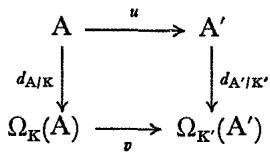
\includegraphics[keepaspectratio]{images/part004_9ff9737d.jpg}}

\(d_{\mathbf{A}^{\prime} / \mathbf{K}^{\prime}}\circ u\) 是 A 的、取值于 A-模 \(\Omega_{\mathbf{K}^{\prime}}(\mathbf{A}^{\prime})\) 的一个 K-导子； \(v\) 的存在性与唯一性随后由第11号命题18得出。

命题19中的映射 v 将记作 \(\Omega(u)\) ；若存在一个由交换环同态构成的交换图

\pandocbounded{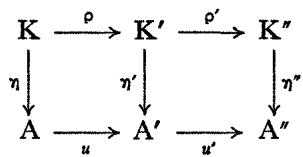
\includegraphics[keepaspectratio]{images/part004_26fbb1e8.jpg}}

由命题19的唯一性性质，立即得出

\[
\Omega (u ^ {\prime} \circ u) = \Omega (u ^ {\prime}) \circ \Omega (u).
\]

由于 \(\Omega_{\mathbf{K}'}(\mathbf{A}')\) 是一个 \(\mathbf{A}'\) -模，由 \(\Omega(u)\) 我们典范地导出一个 \(\mathbf{A}'\) -线性映射

\[
\Omega_ {0} (u): \Omega_ {\mathbf {K}} (\mathrm{A}) \otimes_ {\mathrm{A}} \mathrm{A} ^ {\prime} \rightarrow \Omega_ {\mathbf {K} ^ {\prime}} (\mathrm{A} ^ {\prime})\tag{41}
\]

，使得 \(\Omega(u)\) 是 \(\Omega_0(u)\) 与典范同态 \(i_{\mathbf{A}}: \Omega_{\mathbf{K}}(\mathbf{A}) \to \Omega_{\mathbf{K}}(\mathbf{A}) \otimes_{\mathbf{A}} \mathbf{A}'\) 的复合。对每个 \(\mathbf{A}'\) -模 \(\mathbf{E}'\) ，有一个交换图

\pandocbounded{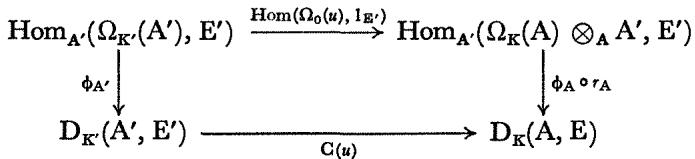
\includegraphics[keepaspectratio]{images/part004_95f64194.jpg}}

（其中 \(\mathbf{C}(u)\) 是映射 \(D \mapsto D \circ u\) （第7号，命题9），而 \(r_{A}\) 是典范同构

\[
\operatorname{Hom} \left(i _ {\mathrm{A}}, 1 _ {\mathrm{E} ^ {\prime}}\right): \operatorname{Hom} _ {\mathrm{A} ^ {\prime}} \left(\Omega_ {\mathrm{K}} (\mathrm{A}) \otimes_ {\mathrm{A}} \mathrm{A} ^ {\prime}, \mathrm{E} ^ {\prime}\right)\rightarrow \operatorname{Hom} _ {\mathrm{A}} \left(\Omega_ {\mathrm{K}} (\mathrm{A}), \mathrm{E} ^ {\prime}\right);
\]

这直接由命题19以及同构 \(\phi_{\mathbf{A}}\) 和 \(\phi_{\mathbf{A}^{\prime}}\) 的定义得出。

命题20. 假设 \(\mathbf{A}' = \mathbf{A} \otimes_{\mathbb{K}} \mathbf{K}'\) ，其中 \(\eta': \mathbf{K}' \to \mathbf{A}'\) 和 \(u: \mathbf{A} \to \mathbf{A}'\) 是典范同态。则 \(\mathbf{A}'\) -线性映射

\[
\Omega_ {0} (u): \Omega_ {\mathbf {K}} (\mathrm{A}) \otimes_ {\mathbf {A}} \mathrm{A} ^ {\prime} \rightarrow \Omega_ {\mathbf {K} ^ {\prime}} (\mathrm{A} ^ {\prime})
\]

是一个同构。

由于图(42)中竖直箭头是双射，问题归结为证明：对每个A'-模E'，图(42)中的同态C(u):D → D ∘ u是双射（II，§2，第1号，定理1）。现在Hom(u, 1\_E') : Hom\_K'(A ⊗\_K K', E') → Hom\_K(A, E')是同构（II，§5，第1号，命题1），而C(u)是它在D\_K'(A', E')上的限制，因此是单射；此外，若 f: A' → E' 是一个 K'-线性映射，使得

\[
f \circ u: \mathrm{A} \rightarrow \mathrm{E} ^ {\prime}
\]

是 K-导子，则由 \(f\) 是 \(\mathbf{K}'\) -线性的以及 \(f((x \otimes 1)(y \otimes 1)) = (y \otimes 1)f(x \otimes 1) + (x \otimes 1)f(y \otimes 1)\) （对 A 中的 \(x, y\) ）这一事实，立即得出 \(f\) 是一个 \(\mathbf{K}'\) -导子，因为元素 \(x \otimes 1\) （对 \(x \in A\) ）构成 \(\mathbf{K}'\) -模 \(A'\) 的一个生成系；这就完成了 \(C(u)\) 是双射的证明。

从现在起，我们把注意力限制在 \(\rho: \mathbf{K} \to \mathbf{K}'\) 是 \(\mathbf{K}\) 的恒等映射的情形；每个 K-代数同态 \(u: \mathbf{A} \to \mathbf{B}\) 因此被映为一个 B-线性映射

\[
\Omega_ {0} (u): \Omega_ {\mathbf {K}} (\mathrm{A}) \otimes_ {\mathbf {K}} \mathrm{B} \rightarrow \Omega_ {\mathbf {K}} (\mathrm{B}).\tag{43}
\]

另一方面，我们可以考虑 A-微分的 B-模 \(\Omega_{\mathbf{A}}(\mathbf{B})\) ，因为 B 通过 u 成为 A-代数；典范导子 \(d_{\mathrm{B/A}}: \mathbf{B} \to \Omega_{\mathbf{A}}(\mathbf{B})\) 当然更是 K-导子，因此它唯一地分解为

\[
\mathbf {B} \xrightarrow {d _ {\mathbf {B} / \mathbf {K}}} \Omega_ {\mathbf {K}} (\mathbf {B}) \xrightarrow {\Omega_ {u}} \Omega_ {\mathbf {A}} (\mathbf {B})
\]

其中 \(\Omega_{u}\) 是 B-线性映射（第11号，命题18）。对每个 B-模 E，有交换图

\[
\begin{array}{c} \operatorname{Hom} _ {\mathbf {B}} (\Omega_ {\mathbf {A}} (\mathbf {B}), \mathrm{E}) \xrightarrow {\operatorname{Hom} (\Omega_ {u} , 1 _ {\mathbf {E}})} \operatorname{Hom} _ {\mathbf {B}} (\Omega_ {\mathbf {K}} (\mathbf {B}), \mathrm{E}) \\ \phi_ {\mathbf {A}, \mathbf {B}} \Biggl \downarrow \\ \mathrm{D} _ {\mathbf {A}} (\mathrm{B}, \mathrm{E}) \xrightarrow [ j _ {u} ]{} \mathrm{D} _ {\mathbf {K}} (\mathrm{B}, \mathrm{E}) \end{array}\tag{44}
\]

其中 \(j_{u}\) 是典范单射（第7号）；这直接由第11号的命题18得出。

命题21：B-线性映射的序列

\[
\Omega_ {\mathbf {K}} (\mathrm{A}) \otimes_ {\mathbf {A}} \mathrm{B} \xrightarrow {\Omega_ {0} (u)} \Omega_ {\mathbf {K}} (\mathrm{B}) \xrightarrow {\Omega_ {u}} \Omega_ {\mathbf {A}} (\mathrm{B}) \to 0\tag{45}
\]

是正合的。

只需验证：对每个B-模E，序列

\[
\begin{array}{c} 0 \to \operatorname{Hom} _ {\mathrm{B}} (\Omega_ {\mathrm{A}} (\mathrm{B}), \mathrm{E}) \xrightarrow {\operatorname{Hom} (\Omega_ {\mathrm{u}} , 1 _ {\mathrm{E}})} \operatorname{Hom} _ {\mathrm{B}} (\Omega_ {\mathrm{K}} (\mathrm{B}), \mathrm{E}) \\ \xrightarrow {\operatorname{Hom} (\Omega_ {0} (u) , 1 _ {\mathrm{E}})} \operatorname{Hom} _ {\mathrm{B}} (\Omega_ {\mathrm{K}} (\mathrm{A}) \otimes_ {\mathrm{A}} \mathrm{B}, \mathrm{E}) \end{array}
\]

是正合的（II，§2，第1号，定理1）；但由于在交换图（42）和（44）中垂直箭头是同构的，只需证明序列

\[
0 \longrightarrow \mathrm{D} _ {\mathrm{A}} (\mathrm{B}, \mathrm{E}) \xrightarrow {j _ {u}} \mathrm{D} _ {\mathrm{K}} (\mathrm{B}, \mathrm{E}) \xrightarrow {\mathrm{C} (u)} \mathrm{D} _ {\mathrm{K}} (\mathrm{A}, \mathrm{E})
\]

是正合的，这正是第7号的命题11。

现在我们考虑 K-代数同态 \(u: \mathbf{A} \to \mathbf{B}\) 是满射的情形；若 \(\mathfrak{J}\) 是其核，则 \(\mathbf{B}\) 同构于 \(\mathbf{A} / \mathfrak{J}\) 。我们考虑典范导子的限制 \(d| \mathfrak{J}: \mathfrak{J} \to \Omega_{\mathbf{K}}(\mathbf{A})\) （其中 \(d = d_{\mathbf{A} / \mathbf{K}}\) ）以及复合 A-线性映射

\[
d ^ {\prime}: \mathfrak {J} \xrightarrow {d | \mathfrak {J}} \Omega_ {\mathrm{K}} (\mathrm{A}) \xrightarrow {i _ {\mathrm{A}}} \Omega_ {\mathrm{K}} (\mathrm{A}) \otimes_ {\mathrm{A}} \mathrm{B}.
\]

那么 \(d^{\prime}(\mathfrak{J}^{2}) = 0\) ，因为，对于 \(x, y\) 在 \(\mathfrak{J}\) ,

\[
d ^ {\prime} (x y) = d (x y) \otimes 1 = (x. d y + y. d x) \otimes 1 = d y \otimes u (x) + d x \otimes u (y) = 0
\]

因为 \(u(x) = u(y) = 0\) 。因此我们由 \(d'\) 通过过渡到商得到一个 A-线性映射

\[
\bar {d} \colon \mathfrak {J} / \mathfrak {J} ^ {2} \rightarrow \Omega_ {\mathrm{K}} (\mathrm{A}) \otimes_ {\mathrm{A}} \mathrm{B}
\]

且由于 \(\mathfrak{J}\) 零化 A-模 \(\mathfrak{J} / \mathfrak{J}^2\) ， \(\bar{d}\) 是一个 B-线性映射。

命题 22。设 \(\mathfrak{J}\) 是交换 K-代数 A 的一个理想，B = A/ \(\mathfrak{J}\) ， \(u:A\to B\) 为典范同态。B-线性映射的序列

\[
\mathfrak {J} / \mathfrak {J} ^ {2} \xrightarrow {\overline {{d}}} \Omega_ {\mathrm{K}} (\mathrm{A}) \otimes_ {\mathrm{A}} \mathrm{B} \xrightarrow {\Omega_ {0} (u)} \Omega_ {\mathrm{K}} (\mathrm{B}) \to 0\tag{46}
\]

因而是正合的。

注意， \(\Omega_{\mathbf{K}}(\mathbf{A}) \otimes_{\mathbf{A}} \mathbf{B}\) 与 \(\Omega_{\mathbf{K}}(\mathbf{A}) / \mathfrak{J} \Omega_{\mathbf{K}}(\mathbf{A})\) 相等同，且 \(\bar{d}\) 的像就是 \(d(\mathfrak{J})\) 在这个商模中的像； \(\Omega_{\mathbf{K}}(\mathbf{A}) \otimes_{\mathbf{A}} \mathbf{B}\) 关于 \(\operatorname{Im}(\bar{d})\) 的商因此等同于商 \(\Omega_{\mathbf{K}}(\mathbf{A}) / \mathbf{N}\) ，其中 \(\mathbf{N}\) 是由 \(\mathfrak{J} \Omega_{\mathbf{K}}(\mathbf{A})\) 和 \(d(\mathfrak{J})\) 生成的子 A-模。此外，复合映射

\[
\mathrm{A} \xrightarrow {d _ {\mathrm{A} / \mathrm{K}}} \Omega_ {\mathrm{K}} (\mathrm{A}) \longrightarrow \Omega_ {\mathrm{K}} (\mathrm{A}) / \mathrm{N}
\]

是一个 K-导子（第7号，命题9），并且由于它在 \(\mathfrak{J}\) 上为零（根据 N 的定义），当过渡到商时，它定义了一个 K-导子 \(D_0:B\to \Omega_{\mathbb{K}}(A) / N\) .

考虑到泛映射问题解的唯一性，可以归结为证明：对于每个 B-模 E 和每个 K-导子 D: B → E，存在唯一的 B-线性映射 g： \(\Omega_{\mathrm{K}}(\mathrm{A})/\mathrm{N} \rightarrow \mathrm{E}\) ，使得 \(D = g \circ D_{0}\) 。但是，复合映射 D ∘ u: A → E 是一个 K-导子（第7号，命题9），因此存在且仅存在一个 A-线性映射 f： \(\Omega_{\mathrm{K}}(\mathrm{A}) \rightarrow \mathrm{E}\) ，使得 \(f \circ d_{A/K} = D \circ u\) 。这个关系式已经表明 f 在 \(d(\mathfrak{J})\) 上为零；又因为 E 是 B-模， \(\mathfrak{J} E = \{0\}\) ，所以 f 在 \(\mathfrak{J} \Omega_{\mathrm{K}}(\mathrm{A})\) 上为零；因此 f 在 N 上为零，并在取商后定义了一个 B-线性映射 g： \(\Omega_{\mathrm{K}}(\mathrm{A})/\mathrm{N} \rightarrow \mathrm{E}\) ，使得 \(g \circ D_{0} = D\) ；g 的唯一性由 f 的唯一性得出。

不要以为，即使 \(u: \mathbf{A} \to \mathbf{B}\) 是单射同态， \(\Omega_0(u): \Omega_{\mathbf{K}}(\mathbf{A}) \otimes_{\mathbf{A}} \mathbf{B} \to \Omega_{\mathbf{K}}(\mathbf{B})\) 也是单射（练习5）。然而我们有如下命题：

命题23。设 A 是一个整 K-代数，B 是其分式域，且 \(u: \mathbf{A} \to \mathbf{B}\) 为典范单射。则 \(\Omega_0(u): \Omega_{\mathbf{K}}(\mathbf{A}) \otimes_{\mathbf{A}} \mathbf{B} \to \Omega_{\mathbf{K}}(\mathbf{B})\) 是一个同构。

利用图(42)中竖直箭头是双射这一事实，问题归结为证明：对于B上的每一个向量空间E，映射 \(\mathrm{C}(u):\mathrm{D}_{\mathrm{K}}(\mathrm{B},\mathrm{E})\to\mathrm{D}_{\mathrm{K}}(\mathrm{A},\mathrm{E})\) 是双射。但这可由以下事实推出：A到E的每一个K-导子都能唯一地延拓为B到E的K-导子（第5号，命题5）。

\section{余代数、多重线性形式的乘积、内乘与对偶}

在本段中，A 是带平凡分次的交换环。对 N 型分次 A-模 M， \(M^{*gr}\) 表示这样的 N 型分次 A-模：其 n 次齐次元素是在 \(M_{k}\) 上（对所有 \(k \neq n\) ）为零的那些 A-线性形式。

\subsection{余代数}

定义 1. A 上的余代数（或 A-余代数，若不致混淆则简称为余代数）是一个集合 E，其结构由给出以下内容来定义：

\begin{enumerate}
\def\labelenumi{(\arabic{enumi})}
\item
  E 上的一个 A-模结构；
\item
  一个 A-线性映射 \(c: \mathbf{E} \to \mathbf{E} \otimes_{\mathbf{A}} \mathbf{E}\) ，称为 \(\mathbf{E}\) 的余积。
\end{enumerate}

定义2. 给定两个余代数E、E'，其余积分别记为c和c'，从E到E'的一个态射是一个A-线性映射u：E → E'，使得

\[
(u \otimes u) \circ c = c ^ {\prime} \circ u\tag{1}
\]

换言之，它使得A-线性映射的图表可交换

\pandocbounded{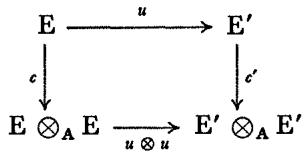
\includegraphics[keepaspectratio]{images/part004_6ed4336b.jpg}}

立即可以验证，恒等映射是态射，两个态射的复合是态射，并且每个双射态射都是同构。

示例。（1）典范同构 \(\mathbf{A} \to \mathbf{A} \otimes_{\mathbf{A}} \mathbf{A}\) (II, § 3, 第 5 号) 在 \(\mathbf{A}\) 上定义了一个 A-余代数结构。

\begin{enumerate}
\def\labelenumi{(\arabic{enumi})}
\setcounter{enumi}{1}
\item
  设 E 为一个余代数，c 为其余积，且 \(\sigma\) 为 A-模 \(E \otimes_{A} E\) 的典范自同构，使得 \(\sigma(x \otimes y) = y \otimes x\) （对 \(x \in E\) , \(y \in E\) ）；A-线性映射 \(\sigma \circ c\) 在 E 上定义了一个新的余代数结构。带此结构的 E 称为给定余代数 E 的反余代数。
\item
  设 B 为一个 A-代数，并设 \(m:B \otimes_{A} B \to B\) 为定义 B 上乘法的 A-线性映射（ \(\S 1\) ，第3号）。转置 \(^{t}m\) 于是是从 A-模 B 的对偶 \(B^{*}\) 到 \((\mathbf{B} \otimes_{\mathbf{A}} \mathbf{B})^{*}\) （即 A-模 \(B \otimes_{A} B\) 的对偶）中的一个 A-线性映射。若 B 还是有限生成的投射 A-模，则典范映射 \(\mu:B^{*} \otimes_{A} B^{*} \to (\mathbf{B} \otimes_{\mathbf{A}} \mathbf{B})^{*}\) 是一个 A-模同构（II， \(\S 4\) ，第4号）；映射 \(c = \mu^{-1} \circ ^{t}m\) 于是是一个余积，它在 A-模 B 的对偶 \(B^{*}\) 上定义了一个余代数结构。
\item
  设 X 是一个集合， \(\mathbf{A}^{(\mathbf{X})}\) 是 X 中元素以 A 中系数构成的形式线性组合的 A-模（II，§1，第11号），且 \((e_{x})_{x\in\mathbf{X}}\) 是 \(\mathbf{A}^{(\mathbf{X})}\) 的典范基。A-线性映射 \(c:A^{(\mathbf{X})}\to\mathbf{A}^{(\mathbf{X})}\otimes_{\mathbf{A}}\mathbf{A}^{(\mathbf{X})}\) 由条件 \(c(e_{x})=e_{x}\otimes e_{x}\) 定义，从而在 \(\mathbf{A}^{(\mathbf{X})}\) 上得到了一个典范余代数结构。
\item
  设 \(\mathbf{M}\) 是一个 A-模，且 \(\mathsf{T}(\mathbf{M})\) 是 \(\mathbf{M}\) 的张量代数 ( \(\S 5\) ，第1号）；根据 II， \(\S 3\) 第9号，存在且仅存在一个 A-线性映射 \(c\) ，它从 A-模 \(\mathsf{T}(\mathbf{M})\) 到 A-模 \(\mathsf{T}(\mathbf{M}) \otimes_{\mathbf{A}} \mathsf{T}(\mathbf{M})\) 中，使得对所有 \(n \geqslant 0\) ，
\end{enumerate}

\[
c (x _ {1} x _ {2} \dots x _ {n}) = \sum_ {0 \leqslant p \leqslant n} (x _ {1} x _ {2} \dots x _ {p}) \otimes (x _ {p + 1} \dots x _ {n})\tag{3}
\]

对所有 \(x_{i} \in \mathbf{M}\) ( \(x_{1}x_{2}\ldots x_{n}\) 表示代数 \(\mathsf{T}(\mathbf{M})\) 中的乘积）。这样， \(\mathsf{T}(\mathbf{M})\) 就被赋予了余代数结构。

\begin{enumerate}
\def\labelenumi{(\arabic{enumi})}
\setcounter{enumi}{5}
\tightlist
\item
  设 M 是一个 A-模，S(M) 是 M 的对称代数（§ 6，第 1 号）；从 M 到 M × M 的对角映射 \(\Delta: x \mapsto (x, x)\) 是一个 A-线性映射，因此对应着从 A-代数 S(M) 到 A-代数 S(M × M) 的一个同态 S(Δ)（§ 6，第 2 号，命题 3）。另一方面，在 § 6，第 6 号中我们定义了一个典范分次代数同构 \(h \colon \mathbb{S}(\mathbf{M} \times \mathbf{M}) \to \mathbb{S}(\mathbf{M}) \otimes_{\mathbf{A}} \mathbb{S}(\mathbf{M})\) ；通过复合，我们因此得到一个 A-代数同态
\end{enumerate}

\[
c = h \circ \mathbf {S} (\Delta): \mathbf {S} (\mathbf {M}) \rightarrow \mathbf {S} (\mathbf {M}) \otimes_ {\mathbf {A}} \mathbf {S} (\mathbf {M}),
\]

从而在 \(\mathbf{S}(\mathbf{M})\) 上定义了一个余代数结构。对所有 \(x\in \mathbf{M}\) ，根据定义 \(\mathbf{S}(\Delta)(x) = (x,x)\) ，而 § 6 第6号中给出的 \(h\) 的定义表明

\[
h ((x, x)) = x \otimes 1 + 1 \otimes x.
\]

由此可得 \(c\) 是唯一的代数同态，使得对所有 \(x \in \mathbf{M}\) ,

\[
c (x) = x \otimes 1 + 1 \otimes x.\tag{4}
\]

由于 \(c\) 是一个代数同态，因此得出：对每个序列 \((x_{i})_{1\leqslant i\leqslant n}\) （ \(n\) 个元素取自 \(\mathbf{M}\) ），

\[
\begin{array}{r l} c (x _ {1} x _ {2} \dots x _ {n}) & = \prod_ {i = 1} ^ {n} (x _ {i} \otimes 1 + 1 \otimes x _ {i}) \\ & = \sum (x _ {i _ {1}} \dots x _ {i _ {p}}) \otimes (x _ {j _ {1}} \dots x _ {j _ {n - p}}) \end{array}\tag{5}
\]

（5）式右端的求和是对所有严格递增序列（在某些情况下为空）的有序对进行的

\[
i _ {1} <   i _ {2} <   \dots <   i _ {p}, \quad j _ {1} <   j _ {2} <   \dots <   j _ {n - p}
\]

的元素组成 \([1, n]\) ，且其元素集合互补。元素 \(c(x_1 x_2 \ldots x_n)\) 是总次数为 \(n\) 的、 \(\mathbb{S}(\mathbf{M}) \otimes_{\mathbf{A}} \mathbb{S}(\mathbf{M})\) 中的元素，其双次数为 \((p, n - p)\) 的分量是

\[
\sum_ {\sigma} \left(x _ {\sigma (1)} \dots x _ {\sigma (p)}\right) \otimes \left(x _ {\sigma (p + 1)} \dots x _ {\sigma (n)}\right)\tag{6}
\]

其中求和遍历所有排列 \(\sigma\in\mathbb{S}_{n}\) ，这些排列在每个区间 \([1,p]\) 和 \([p+1,n]\) 上都是递增的。

\begin{enumerate}
\def\labelenumi{(\arabic{enumi})}
\setcounter{enumi}{6}
\tightlist
\item
  设 \(\mathbf{M}\) 是一个 A-模，对外代数 \(\bigwedge (\mathbf{M})\) 按照例 6 中对 \(\mathbb{S}(\mathbf{M})\) 的方式处理；对角映射 \(\Delta : \mathbf{M} \to \mathbf{M} \times \mathbf{M}\) 这次定义了同态 \(\bigwedge (\Delta)\) ，它从 A-代数 \(\bigwedge (\mathbf{M})\) 到 A-代数 \(\bigwedge (\mathbf{M} \times \mathbf{M})\) 中（§7，第2号，命题2）；另一方面，存在典范分次代数同构
\end{enumerate}

\[
h: \bigwedge (\mathbf {M} \times \mathbf {M}) \rightarrow \bigwedge (\mathbf {M}) ^ {\mathrm{g}} \otimes_ {\mathbf {A}} \bigwedge (\mathbf {M})
\]

（§7，第7号，命题10），因此通过复合得到代数同态 \(c = h \circ \bigwedge(\Delta): \bigwedge(M) \to \bigwedge(M)^{\mathfrak{g}} \otimes_{A} \bigwedge(M)\) ，它可视为 A-模同态 \(\bigwedge(M) \to \bigwedge(M) \otimes_{A} \bigwedge(M)\) ，从而在 \(\bigwedge(M)\) 上定义了一个余代数结构。可如同例 6 那样证明 \(c\) 是唯一的代数同态，使得对所有 \(x \in M\) ，

\[
c (x) = x \otimes 1 + 1 \otimes x,\tag{7}
\]

，因此，对每个序列 \((x_{i})_{1\leqslant i\leqslant n}\) （元素属于 \(\mathbf{M}\) ），

\[
c \left(x _ {1} \wedge x _ {2} \wedge \dots \wedge x _ {n}\right) = \left(x _ {1} \otimes 1 + 1 \otimes x _ {1}\right) \wedge \dots \wedge \left(x _ {n} \otimes 1 + 1 \otimes x _ {n}\right)
\]

其中右侧的乘积是在代数中进行的

\[
\Lambda (\mathbf {M}) ^ {\mathfrak {g}} \otimes_ {\mathbf {A}} \Lambda (\mathbf {M});
\]

为了计算这个乘积，对每对严格递增序列 \(i_1 < i_2 < \cdots < i_p\) , \(j_1 < j_2 < \cdots < j_{n-p}\) （由 \([1, n]\) 的元素组成，且其元素集合互补），考虑乘积 \(y_1y_2\ldots y_n\) ，其中 \(y_{i_h} = x_{i_h} \otimes 1 (1 \leqslant h \leqslant p)\) 和 \(y_{j_k} = 1 \otimes x_{j_k} (1 \leqslant k \leqslant n - p)\) 并且求和是对所有这些乘积进行的。由于分次代数 \(\bigwedge (\mathbf{M})^{\mathfrak{g}} \otimes_{\mathbf{A}} \bigwedge (\mathbf{M})\) 是反交换的，且元素 \(x_i \otimes 1\) 和 \(1 \otimes x_i\) 的总次数为1，根据§4，第6号，引理3和引理1，

\[
\begin{array}{r l} c (x _ {1} \wedge x _ {2} \wedge \dots \wedge x _ {n}) & = \sum (- 1) ^ {\nu} (x _ {i _ {1}} \wedge \dots \wedge x _ {i _ {p}}) \otimes (x _ {j _ {1}} \wedge \dots \wedge x _ {j _ {n - p}}) \end{array} \tag {8}
\]

其中 v 是有序对 \((h, k)\) 的个数，这些对满足 \(j_{k} < i_{h}\) ，且求和范围与 (5) 中相同。元素 \(c(x_{1} \wedge \cdots \wedge x_{n})\) 在 \(\bigwedge(\mathbf{M})^{\mathbf{g}} \otimes_{\mathbf{A}} \bigwedge(\mathbf{M})\) 中的总次数为 n，其双次数 \((p, n - p)\) 的齐次分量等于

\[
\sum_ {\sigma} \varepsilon_ {\sigma} (x _ {\sigma (1)} \wedge \dots \wedge x _ {\sigma (p)}) \otimes (x _ {\sigma (p + 1)} \wedge \dots \wedge x _ {\sigma (n)})\tag{9}
\]

求和遍历所有置换 \(\sigma\in\mathfrak{S}_{n}\) ，它们在每个区间 \([1,p]\) 和 \([p+1,n]\) 上都是递增的。

今后当我们谈到 \(\mathbf{A}^{(\mathbf{X})}\) , \(\mathsf{T}(\mathbf{M})\) , \(\mathsf{S}(\mathbf{M})\) 或 \(\bigwedge (\mathbf{M})\) 作为余代数时，除非另有说明，我们指的是分别在例 4、5、6 和 7 中定义的余代数结构。

\begin{enumerate}
\def\labelenumi{(\arabic{enumi})}
\setcounter{enumi}{7}
\tightlist
\item
  设 E, F 为两个 A-余代数，c, \(c'\) 分别为其余积。设 \(\tau:(\mathbf{E} \otimes_{\mathbf{A}} \mathbf{E}) \otimes_{\mathbf{A}} (\mathbf{F} \otimes_{\mathbf{A}} \mathbf{F}) \to (\mathbf{E} \otimes_{\mathbf{A}} \mathbf{F}) \otimes_{\mathbf{A}} (\mathbf{E} \otimes_{\mathbf{A}} \mathbf{F})\) 表示结合性同构，使得 \(\tau((x \otimes x') \otimes (y \otimes y')) = (x \otimes y) \otimes (x' \otimes y')\) 对 E 中的 \(x, x'\) 和 F 中的 \(y, y'\) 成立。则复合线性映射
\end{enumerate}

\[
\mathrm{E} \otimes_ {\mathrm{A}} \mathrm{F} \xrightarrow {c \otimes c ^ {\prime}} (\mathrm{E} \otimes_ {\mathrm{A}} \mathrm{E}) \otimes_ {\mathrm{A}} (\mathrm{F} \otimes_ {\mathrm{A}} \mathrm{F}) \xrightarrow {\tau} (\mathrm{E} \otimes_ {\mathrm{A}} \mathrm{F}) \otimes_ {\mathrm{A}} (\mathrm{E} \otimes_ {\mathrm{A}} \mathrm{F})
\]

在 A-模 E \(\otimes_{\mathbf{A}}\mathbf{F}\) 上定义了一个余代数结构，称为余代数 E 和 F 的张量积。

设 E 为一个余代数， \(\Delta\) 为一个交换幺半群。A-模 E 上的分次 \((\mathrm{E}_{\lambda})_{\lambda\in\Delta}\) 称为与 E 的余积 c 相容，如果 c 是从分次 A-模 E 到分次 A-模（ \(\Delta\) 型的 \(E\otimes_{A}E\) ）中的 0 次分次同态，换言之（II，§11，第 5 号），如果

\[
\mathrm{c} (\mathrm{E} _ {\lambda}) \subset \sum_ {\mu + \nu = \lambda} \mathrm{E} _ {\mu} \otimes_ {\mathbf {A}} \mathrm{E} _ {\nu}.\tag{10}
\]

在下文中，我们通常将注意力限制在与余积相容的 N 型分次上；带有这种分次的余代数也称为分次余代数。若 F 是另一个分次余代数，则分次余代数态射 \(\phi:E\to F\) 按定义是一个余代数态射（定义 2），同时也是分次 A-模之间的 0 次分次同态。

例。（9）显然，上述定义的余代数 \(\mathsf{T}(\mathbf{M})\) , \(\mathsf{S}(\mathbf{M})\) 和 \(\bigwedge (\mathbf{M})\) 都是分次余代数。

\subsection{余结合性、余交换性、余单位}

设 E 为一个余代数，c 为其余积，N, N', N'' 为三个 A-模，m 为 N × N' 到 N'' 的一个双线性映射。设 \(\tilde{m}:N \otimes_{A} N' \to N''\) 为对应于 m 的 A-线性映射。若 \(u:E \to N\) , \(v:E \to N'\) 是两个 A-线性映射，我们得到一个 A-线性映射 \(u \otimes v:E \otimes_{A} E \to N \otimes_{A} N'\) 以及一个从 E 到 N'' 的复合 A-线性映射：

\[
m (u, v): \mathrm{E} \xrightarrow {c} \mathrm{E} \otimes_ {\mathrm{A}} \mathrm{E} \xrightarrow {u \otimes v} \mathrm{N} \otimes_ {\mathrm{A}} \mathrm{N} ^ {\prime} \xrightarrow {\tilde {m}} \mathrm{N} ^ {\prime \prime}.\tag{11}
\]

显然，我们由此定义了一个 A-双线性映射 \((u, v) \mapsto m(u, v)\) ，它从 \(\operatorname{Hom}_{\mathbf{A}}(\mathbf{E}, \mathbf{N}) \times \operatorname{Hom}_{\mathbf{A}}(\mathbf{E}, \mathbf{N}')\) 到 \(\operatorname{Hom}_{\mathbf{A}}(\mathbf{E}, \mathbf{N}'')\) 中。

当 E 为分次余代数，N, N', N'' 为同类型的分次 A-模，且 \(\tilde{m}\) 为从 N \(\otimes_{A}N'\) 到 N'' 的 k 次分次同态时，若 u（相应地 v）是 p 次（相应地 q 次）分次同态，则 \(m(u,v)\) 是次数为 \(p + q + k\) 的分次同态。

例。（1）取 E 为分次余代数 T(M)（第 1 号），并假设 N, N', N'' 具有平凡分次。则从 T(M) 到 N（相应地 N', N''）的 -p 次分次同态对应于从 M\^{}p 到 N（相应地 N', N''）的多重线性映射。给定一个多重线性映射 u: M\^{}p → N 和一个多重线性映射 v: M\^{}q → N'，上述方法使我们能够推导出一个多重线性映射 m(u, v)：M\^{}\{p+q\} → N''，称为u与v的（关于m的）乘积。公式（3）（第1号）和（11）表明，对于M中的x\_1, . . ., x\_p+q，

\[
(m (u, v)) \left(x _ {1}, \dots , x _ {p + q}\right) = m \left(u \left(x _ {1}, \dots , x _ {p}\right), v \left(x _ {p + 1}, \dots , x _ {p + q}\right)\right).
\]

\begin{enumerate}
\def\labelenumi{(\arabic{enumi})}
\setcounter{enumi}{1}
\tightlist
\item
  设 E 为分次余代数 S(M)（第 1 号），对 N、N'、N'' 保持相同的假设。从 S(M) 到 N 的 −p 次分次同态对应于从 M \(^{p}\) 到 N 的对称多重线性映射（§ 6，第 3 号）。于是，由对称多重线性映射 u: M \(^{p}\) → N 和对称多重线性映射 v: M \(^{q}\) → N' 得到一个对称多重线性映射 m(u, v)：M \(^{p+q}\) → N''，也（为避免混淆）记作 \(u \cdot_{m} v\) （甚至 \(u \cdot v\)），并称为 u 和 v 的（关于 m 的）对称积。公式 (6)（第 1 号）和 (11) 表明，对于 M 中的 x₁， \ldots， \(_{p+q}\) ，
\end{enumerate}

\[
(u \cdot_{m} v) (x _ {1}, \dots , x _ {p + q}) = \sum_ {\sigma} m (u (x _ {\sigma (1)}, \dots , x _ {\sigma (p)}), v (x _ {\sigma (p + 1)}, \dots , x _ {\sigma (p + q)}))
\]

求和遍历所有置换 \(\sigma\in\mathfrak{S}_{p+q}\) ，这些置换在每个区间 \([1,p]\) 和 \([p+1,p+q]\) 上都是递增的。

\begin{enumerate}
\def\labelenumi{(\arabic{enumi})}
\setcounter{enumi}{2}
\tightlist
\item
  取 E 为分次余代数 \(\bigwedge (\mathbf{M})\) （第 1 号）。于是我们类似地从交错多重线性映射 \(u: \mathbf{M}^p \to \mathbf{N}\) 和交错多重线性映射 \(v: \mathbf{M}^q \to \mathbf{N}'\) 得到一个交错多重线性映射 \(m(u, v): \mathbf{M}^{p + q} \to \mathbf{N}''\) ，也记作 \(u \wedge_m v\) 或 \(u \wedge v\) ，并称为（关于 \(m\) 的） \(u\) 和 \(v\) 的交错积。公式（9）（第 1 号）和（11）表明在这种情况下，对于 \(x_1, \ldots, x_{p + q}\) （在 \(\mathbf{M}\) 中），
\end{enumerate}

\[
(u \wedge_ {m} v) (x _ {1}, \dots , x _ {p + q}) = \sum_ {\sigma} \varepsilon_ {\sigma} m (u (x _ {\sigma (1)}, \dots , x _ {\sigma (p)}), v (x _ {\sigma (p + 1)}, \dots , x _ {\sigma (p + q)}))
\]

求和再次遍历所有排列 \(\sigma \in \mathfrak{S}_{p + q}\) ，这些排列在每个区间 \([1, p]\) 和 \([p + 1, p + q]\) 上都是递增的。

我们回到 E 为任意分次余代数（N 型）的情形，并假设三个模 N、N'、N'' 都等于一个 Z 型分次 A-代数 B 的底层 A-模，映射 m 为 B 中的乘法，从而 \(\tilde{m}:B\otimes_{A}B\to B\) 是一个次数为 0 的分次 A-线性映射。于是在分次 A-模 \(\operatorname{Homgr}_{A}(E,B)=C\) 上获得了一个分次 A-代数结构。

特别地，假设 B = A（具有平凡分次），因此 \(\operatorname{Homgr}_{\mathbf{A}}(\mathbf{E}, \mathbf{A})\) 是分次对偶 \(E^{*gr}\) ，从而它具有一个分次 A-代数结构。

设 F 为另一个分次余代数， \(c'\) 为其余积， \(\phi:E\to F\) 为一个分次余代数态射（第1号）；则典范分次态射

\[
\tilde {\phi} = \operatorname{Hom} (\phi , 1 _ {B}): \operatorname{Homgr} _ {A} (F, B) \rightarrow \operatorname{Homgr} _ {A} (E, B)
\]

是一个分次代数同态。对于 \(u, v\) 在 \(\operatorname{Homgr}_{\mathbf{A}}(\mathbf{F}, \mathbf{B})\) 和 \(x \in \mathbf{E}\) ,

\[
(\tilde {\phi} (u v)) (x) = (u v) (\phi (x)) = m ((u \otimes v) (c ^ {\prime} (\phi (x))))
\]

但根据假设 \(c'(\phi(x)) = (\phi \otimes \phi)(c(x))\) ，因此

\[
(u \otimes v) (c ^ {\prime} (\phi (x))) = (\tilde {\phi} (u) \otimes \tilde {\phi} (v)) (c (x))
\]

，从而 \(\tilde{\phi}(uv) = \tilde{\phi}(u)\tilde{\phi}(v)\) ，这证明了我们的断言。

特别地，分次转置 \({}^{t}\phi: \mathrm{F}^{*gr} \to \mathrm{E}^{*gr}\) 是分次代数同态。

注：假设诸 \(E_{p}\) 是有限生成的投射 A-模，因此分次 A-模（ \(E \otimes_{A} E)^{*gr}\) 和 \(E^{*gr} \otimes_{A} E^{*gr}\) 可以典范地等同（II，§4，第4号，命题4的推论1）。如果 A-模 \(A \otimes_{A} A\) 和 A 也被典范地等同（II，§3，第4号），则线性映射 \(E^{*gr} \otimes_{A} E^{*gr} \to E^{*gr}\) （它定义了 \(E^{*gr}\) 中的乘法）可称为余积 c 的分次转置。

命题1. 设 E 是 A 上的余代数。为使对每个结合 A-代数 B，A-代数 \(\operatorname{Hom}_{\mathbf{A}}(\mathbf{E}, \mathbf{B})\) 是结合的，其充分必要条件是余积 \(c: \mathbf{E} \to \mathbf{E} \otimes_{\mathbf{A}} \mathbf{E}\) 使得图表

\begin{enumerate}
\def\labelenumi{(\arabic{enumi})}
\setcounter{enumi}{11}
\tightlist
\item
\end{enumerate}

\pandocbounded{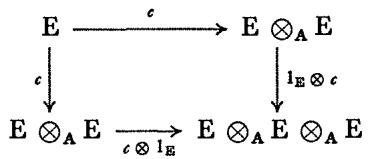
\includegraphics[keepaspectratio]{images/part004_a79ed2ff.jpg}}

是交换的。

设 B 是一个结合 A-代数，且 u、v、w 是 \(\mathbf{C} = \operatorname{Hom}_{\mathbf{A}}(\mathbf{E}, \mathbf{B})\) 的三个元素。设 \(m_{3}\) 表示 A-线性映射 \(B \otimes_{A} B \otimes_{A} B \to B\) ，它把 \(b \otimes b' \otimes b''\) 映为 \(bb'b''\) 。根据代数 C 上乘积的定义， \((uv)w\) 是复合映射

\[
\mathrm{E} \xrightarrow {c} \mathrm{E} \otimes \mathrm{E} \xrightarrow {c \otimes 1 _ {\mathrm{E}}} \mathrm{E} \otimes \mathrm{E} \otimes \mathrm{E} \xrightarrow {u \otimes v \otimes w} \mathrm{B} \otimes \mathrm{B} \otimes \mathrm{B} \xrightarrow {m _ {3}} \mathrm{B}
\]

而 \(u(vw)\) 是复合映射，

\[
\mathrm{E} \xrightarrow {c} \mathrm{E} \otimes \mathrm{E} \xrightarrow {1 _ {\mathrm{E}} \otimes c} \mathrm{E} \otimes \mathrm{E} \otimes \mathrm{E} \xrightarrow {u \otimes v \otimes w} \mathrm{B} \otimes \mathrm{B} \otimes \mathrm{B} \xrightarrow {m _ {3}} \mathrm{B}.
\]

由此可知，若图表 (12) 可交换，则代数 \(\operatorname{Hom}_{\mathbf{A}}(\mathbf{E}, \mathbf{B})\) 对每个结合的A-代数B都是结合的。为建立其逆命题，只需证明存在一个结合的A-代数B以及三个A-线性映射 \(u, v, w\) 将E映入B，使得该映射 \(m_3 \circ (u \otimes v \otimes w)\) 从 \(\mathbf{E} \otimes \mathbf{E} \otimes \mathbf{E}\) 到 B 中是单射。取 B 为 A-代数 \(\mathsf{T}(\mathbf{E})\) ， \(u, v, w\) 为 E 到 \(\mathsf{T}(\mathbf{E})\) 的典范映射。该映射 \(m_3 \circ (u \otimes v \otimes w)\) 就是典范映射 \(\mathbf{E} \otimes \mathbf{E} \otimes \mathbf{E} = \mathsf{T}^3(\mathbf{E}) \to \mathsf{T}(\mathbf{E})\) ，它是单射的。

当余代数 E 满足命题 1 的条件时，称其为余结合的。

例子。(4) 容易直接验证，余代数 A（第 1 号，例 (1)）以及余代数 \(\mathbf{A}^{(\mathbf{X})}\) （第1号，例4）和余代数 \(\mathbf{T}(\mathbf{M})\) （第1号，例5）是余结合的。若B是一个结合A-代数，且是有限生成的投射A-模，则余代数 \(\mathbf{B}^*\) （第1号，例3）是余结合的：因为此时图(12)的交换性可由表达B的结合性的图的交换性通过转置得到（ \(\S\) 1，第3号）。反之，同样的论证以及 A-模 B 与其双对偶的典范等同（II，§2，第7号，命题13的推论4）表明，若余代数 \(\mathbf{B}^*\) 是余结合的，则代数 \(\mathbf{B}\) 是结合的。最后，余代数 \(\mathsf{S}(\mathbf{M})\) 和 \(\bigwedge (\mathbf{M})\) （第1号，例6和7）是余结合的；这由图

\[
\begin{array}{c} \mathrm{M} \xrightarrow {\Delta} \mathrm{M} \times \mathrm{M} \\ \Delta \Biggl \downarrow \\ \mathrm{M} \times \mathrm{M} \xrightarrow [ \Delta \times 1 _ {\mathrm{M}} ]{} \mathrm{M} \times \mathrm{M} \times \mathrm{M} \end{array}
\]

的交换性以及 \(\mathsf{S}(\mathbf{M})\) ( \(\S 6\) ，第2号）和 \(\bigwedge (\mathbf{M})\) ( \(\S 7\) ，第2号）的函子性质得出，它们给出相应的交换图

\[
\left\{ \begin{array}{c} \mathsf {S} (\mathbf {M}) \xrightarrow {\mathsf {S} (\Delta)} \mathsf {S} (\mathbf {M} \times \mathbf {M}) \\ \mathsf {S} (\Delta) \Biggl \downarrow \qquad \qquad \qquad \qquad \qquad \qquad \qquad \qquad \qquad \qquad \qquad \qquad \qquad \qquad \qquad \qquad \qquad \qquad \qquad \qquad \qquad \qquad \qquad \qquad \qquad \qquad \qquad \qquad \qquad \qquad \qquad \qquad \qquad \qquad \mathsf {S} (1 _ {\mathbf {M}} \times \Delta) \\ \mathsf {S} (\mathbf {M} \times \mathbf {M}) \xrightarrow [ \mathsf {S} (\Delta \times 1 _ {\mathbf {M}}) ]{\mathsf {S} (\Delta \times 1 _ {\mathbf {M}})} \mathsf {S} (\mathbf {M} \times \mathbf {M} \times \mathbf {M}) \\ \bigwedge (\mathbf {M}) \xrightarrow {\bigwedge (\Delta)} \bigwedge (\mathbf {M} \times \mathbf {M}) \\ \bigwedge (\Delta) \Biggl \downarrow \qquad \qquad \qquad \qquad \qquad \qquad \qquad \qquad \qquad \qquad \qquad \qquad \qquad \bigwedge (1 _ {\mathbf {M}} \times \Delta) \\ \bigwedge (\mathbf {M} \times \mathbf {M}) \xrightarrow [ \bigwedge (\Delta \times 1 _ {\mathbf {M}}) ]{\bigwedge (\Delta \times 1 _ {\mathbf {M}})} \bigwedge (\mathbf {M} \times \mathbf {M} \times \mathbf {M}) \end{array} \right.\tag{14}
\]

以及直和的对称代数和外代数的典范同构的存在性和函子性（§6，第6号和§7，第7号）。

命题2. 设E是A上的余代数。为了使对于每个交换A-代数B，A-代数 \(\operatorname{Hom}_{\mathbf{A}}(\mathbf{E}, \mathbf{B})\) 是交换的，必要且充分条件是余积 \(c: \mathbf{E} \to \mathbf{E} \otimes_{\mathbf{A}} \mathbf{E}\) 使得图表

\begin{enumerate}
\def\labelenumi{(\arabic{enumi})}
\setcounter{enumi}{14}
\tightlist
\item
\end{enumerate}

\pandocbounded{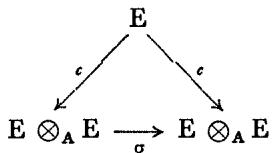
\includegraphics[keepaspectratio]{images/part004_07c99209.jpg}}

(其中 \(\sigma\) 是对称同态，使得 \(\sigma(x \otimes y) = y \otimes x\) ）是交换的（换句话说，只需余代数 E 与其反余代数（第1号，例2）相同即可）。

设 B 是交换 A-代数，u，v 是 C = Hom\_A(E, B) 的两个元素。

根据C中乘积的定义，uv和vu分别等于复合映射

\[
\mathrm{E} \xrightarrow {c} \mathrm{E} \otimes \mathrm{E} \xrightarrow {u \otimes v} \mathrm{B} \otimes \mathrm{B} \xrightarrow {m} \mathrm{B}
\]

和

\[
\mathrm{E} \xrightarrow {c} \mathrm{E} \otimes \mathrm{E} \xrightarrow {v \otimes u} \mathrm{B} \otimes \mathrm{B} \xrightarrow {m} \mathrm{B}.
\]

由此可知，若图(15)可交换，则代数 \(\operatorname{Hom}_{\mathbf{A}}(\mathbf{E}, \mathbf{B})\) 对每个可交换的A-代数B都是可交换的。为建立其逆命题，只需证明存在一个可交换的A-代数B以及两个A-线性映射 \(u, v\) 从 E 到 B 的映射，使得 \(m \circ (u \otimes v): \mathbf{E} \otimes \mathbf{E} \to \mathbf{B}\) 是单射。取 B 为代数 \(\mathsf{S}(\mathbf{E} \oplus \mathbf{E})\) ， \(u\) （相应地 \(v\) ）为典范映射 \(\mathbf{E} \oplus \mathbf{E} \to \mathsf{S}(\mathbf{E} \oplus \mathbf{E})\) 与映射 \(x \mapsto (x, 0)\) （相应地 \(x \mapsto (0, x)\) ）的复合，后者把 E 映入 \(\mathbf{E} \oplus \mathbf{E}\) 。若 \(h: \mathsf{S}(\mathbf{E}) \otimes \mathsf{S}(\mathbf{E}) \to \mathsf{S}(\mathbf{E} \otimes \mathbf{E})\) 是典范同构（ \(\S 6\) ，第6号，命题9）且 \(\lambda: \mathbf{E} \to \mathsf{S}(\mathbf{E})\) 是典范映射，那么 \(h^{-1} \circ m \circ (u \otimes v) = \lambda \otimes \lambda\) 。现在 \(\lambda \otimes \lambda\) 是单射的，因为 \(\lambda(\mathbf{E})\) 是 \(\mathsf{S}(\mathbf{E})\) 的直因子（II，§ 3，第7号，命题7的推论5）。

当余代数 E 满足命题2的条件时，称其为余交换的。

例子。（5）立即可以看出，余代数 A（第1号，例1）和余代数 \(\mathbf{A}^{(\mathbf{X})}\) （II，§ 11，第1号，例4）是余交换的。由第1号的公式（5）可知，余代数 S(M) 是余交换的。最后，对于 A-代数 B，使得 A-模 B 是投射的且有限生成的，要使余代数 \(\mathbf{B}^*\) （第1号，例3）是余交换的，其充分必要条件是 B 是交换的；因为（利用 A-模 B 与其双对偶的典范等同（II，§ 2，第7号）），这由图表（14）的交换性通过转置等价于表达 B 的交换性的图表（§ 1，第3号）这一事实得出。

命题3。设 E 是 A 上的一个余代数。为了使对于每个含单位元的 A-代数 B，A-代数 \(\operatorname{Hom}_{\mathbf{A}}(\mathbf{E},\mathbf{B})\) 是单位的，必要且充分条件是存在 E 上的一个线性形式 \(\gamma\) 使图表（16）交换

\begin{enumerate}
\def\labelenumi{(\arabic{enumi})}
\setcounter{enumi}{15}
\tightlist
\item
\end{enumerate}

\pandocbounded{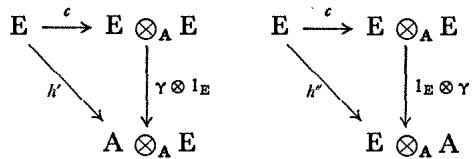
\includegraphics[keepaspectratio]{images/part004_cc0e83d1.jpg}}

（其中 \(c: \mathbf{E} \to \mathbf{E} \otimes_{\mathbf{A}} \mathbf{E}\) 是余积，并且 \(h'\) 和 \(h''\) 是典范同构（II，§ 3，第4号，命题4）。 \(\operatorname{Hom}_{\mathbf{A}}(\mathbf{E}, \mathbf{B})\) 的单位元则是线性映射 \(x \mapsto \gamma(x)1\) （其中1表示B的单位元）。

设 \(\gamma\) 是 E 上的一个线性形式，使得图表（16）交换。设 B 是带单位元 1 的含单位元 A-代数， \(\eta: \mathbf{A} \to \mathbf{B}\) 为典范映射， \(v = \eta \circ \gamma\) 为 A-代数 \(\mathbf{C} = \operatorname{Hom}_{\mathbf{A}}(\mathbf{E}, \mathbf{B})\) 的元素。对于每个元素 \(u \in \mathbf{C}\) ， \(uv\) 是复合映射

\[
\mathrm{E} \xrightarrow {c} \mathrm{E} \otimes \mathrm{E} \xrightarrow {1 _ {\mathrm{E}} \otimes \gamma} \mathrm{E} \otimes \mathrm{A} \xrightarrow {u \otimes \eta} \mathrm{B} \otimes \mathrm{B} \xrightarrow {m} \mathrm{B}.\tag{17}
\]

那么 \(uv = m \circ (u \otimes \eta) \circ h'' = u\) 。类似地可证明 \(vu = u\) ，因此 \(v\) 是 C 的单位元。反之，设 A-模 A ⊕ E 被赋予一个含单位元的代数结构，使得 \((a, x)(a', x') = (aa', ax' + a'x)\) （对 A 中的 \(a, a'\) 和 E 中的 \(x, x'\) ）。设 B 表示如此定义的 A-代数，并设 C 为 A-代数 Hom \(_A(E, B)\) 。假设 C 是含单位元的，并设 \(e: x \mapsto (\gamma(x), \lambda(x))\) 为其单位元（其中 \(\gamma(x) \in A\) 和 \(\lambda(x) \in E\) ）。另一方面，设 \(f\) 是 C 的元素 \(x \mapsto (0, x)\) 。直接计算表明 \(fe\) 是元素

\[
x \mapsto (0, (h ^ {\prime \prime}) ^ {- 1} ((1 _ {E} \otimes \gamma) (c (x))))
\]

此元素属于 C 。条件 \(fe = f\) 蕴含 (16) 中第二个图的交换性，并且类似地可看出条件 \(ef = f\) 蕴含 (16) 中第一个图的交换性。

E 上使图 (16) 交换的线性形式 \(\gamma\) 称为余代数 E 的余单位。一个余代数至多有一个余单位：因为它就是代数 \(\operatorname{Hom}_{\mathbf{A}}(\mathbf{E}, \mathbf{A})\) 的单位元。带有余单位的余代数称为余单位的。

例子。(6) 恒等映射是余代数 A 的余单位；在余代数 \(\mathbf{A}^{(\mathbf{X})}\) （第 1 号，例 4）上，线性形式 \(\gamma\) （使得 \(\gamma(e_x) = 1\) 对所有 \(x \in \mathbf{X}\) 成立）是余单位。在余代数 \(\mathbf{T}(\mathbf{M})\) （相应地 \(\mathbf{S}(\mathbf{M}), \bigwedge(\mathbf{M})\) ）上，线性形式 \(\gamma\) （满足 \(\gamma(1) = 1\) 且 \(\gamma(z) = 0\) ，其中 \(z\) 属于 \(\mathbf{T}^n(\mathbf{M})\) （相应地 \(\mathbf{S}^n(\mathbf{M}), \bigwedge^n(\mathbf{M})\) ）， \(n \geqslant 1\) ）是余单位。最后，设 B 是一个 A-代数，它是有限生成的投射 A-模，并且有单位元 \(e\) ；则在余代数 \(\mathbf{B}^*\) （第1号，例3）上，线性形式 \(\gamma: x^* \mapsto \langle e, x^* \rangle\) 是余单位，因为这个形式恰好是从 A 到 B 的 A-线性映射 \(\eta_e: \xi \mapsto \xi e\) 的转置，并且通过转置，图（16）的交换性可由那些表达（利用 \(\eta_e\) ）"\(e\) 是 B 的单位元"这一事实的图的交换性推出（ \(\S 1\) ，第 3 号）；同样的论证还表明，反之，若余代数 \(\mathbf{B}^*\) 具有一个余单位 \(\gamma\) ，则 \(\gamma\) 的转置定义 B 的单位元 \(e = {}^t\gamma(1)\) 。

命题 4. 设 E 是一个具有余单位 \(\gamma\) 的余代数，并假设 E 中存在一个元素 \(e\) ，使得 \(\gamma(e) = 1\) ；则 E 是子 A-模 Ae 与 \(\mathrm{E}_{\gamma} = \mathrm{Ker}(\gamma)\) 的直和，且

\[
c (e) \equiv e \otimes e (\mathrm{mod.} \mathrm{E} _ {\gamma} \otimes \mathrm{E} _ {\gamma})\tag{18}
\]

\[
\left\{c (x) \equiv x \otimes e + e \otimes x (\mathrm{mod.} \mathrm{E} _ {\gamma} \otimes \mathrm{E} _ {\gamma}) \quad \text { for all } x \in \mathrm{E} _ {\gamma}. \right.
\]

第一个断言是直接的，因为 \(\gamma(x - \gamma(x)e) = 0\) 以及关系 \(\gamma(\alpha e) = 0\) 蕴含 \(\alpha = 0\) 。设 \(c(e) = \sum_{i} s_i \otimes t_i\) ，使得

\[
e = \sum_ {i} \gamma (s _ {i}) t _ {i} = \sum_ {i} \gamma (t _ {i}) s _ {i}
\]

由 (16) 及 \(1 = \gamma(e) = \sum_{i} \gamma(s_i) \gamma(t_i)\) 得出。因此

\[
\begin{array}{r l} \sum_ {i} (s _ {i} - \gamma (s _ {i}) e) \otimes (t _ {i} - \gamma (t _ {i}) e) & = \sum_ {i} s _ {i} \otimes t _ {i} - \sum_ {i} e \otimes \gamma (s _ {i}) t _ {i} \\ & - \sum_ {i} \gamma (t _ {i}) s _ {i} \otimes e \\ & + \sum_ {i} \gamma (s _ {i}) e \otimes \gamma (t _ {i}) e \end{array}
\]

而根据上述关系，这正好是 \(c(e) - e \otimes e\) ；因此这证明了 (18) 中的第一个关系。另一方面，E \(\otimes\) E 作为直和的分解

\[
\mathbf {A} (e \otimes e) \oplus ((\mathbf {A} e) \otimes \mathbf {E} _ {\gamma}) \oplus (\mathbf {E} _ {\gamma} \otimes (\mathbf {A} e)) \oplus (\mathbf {E} _ {\gamma} \otimes \mathbf {E} _ {\gamma})
\]

使得我们可以写出，对于 \(x \in \mathbf{E}_{\gamma}\) , \(c(x) = \lambda(e \otimes e) + (e \otimes y) + (z \otimes e) + u\) （其中 \(u = \sum_{j} v_{j} \otimes w_{j}, y, z\) ，而 \(v_{j}\) 和 \(w_{j}\) 属于 \(\mathbf{E}_{\gamma}\) ）。余单位 \(\gamma\) 的定义随后给出 \(x = \lambda e + y = \lambda e + z\) ，并且由于 \(\gamma(x) = 0\) ，必然有 \(\lambda = 0, x = y = z\) ，由此得出 (18) 的第二个关系式。

注记。设 C 是一个有余单位的余结合 A-余代数，B 是一个含单位元的结合 A-代数，M 是一个左 B-模。A-双线性映射 \((b, m) \mapsto bm\) （从 \(B \times M\) 到 M 中）定义了一个 A-双线性映射

\[
\operatorname{Hom} _ {\mathbf {A}} (\mathrm{C}, \mathrm{B}) \times \operatorname{Hom} _ {\mathbf {A}} (\mathrm{C}, \mathrm{M}) \rightarrow \operatorname{Hom} _ {\mathbf {A}} (\mathrm{C}, \mathrm{M})
\]

这通过本号开头所述的一般程序完成。可以立即验证，该映射在 \(\operatorname{Hom}_{\mathbf{A}}(\mathbf{C}, \mathbf{M})\) 上定义了环 \(\operatorname{Hom}_{\mathbf{A}}(\mathbf{C}, \mathbf{B})\) 上的一个左模结构。

\subsection{N型分次余代数的性质}

命题5. (i) 设 E 是一个具有余单位 \(\gamma\) 的分次余代数；则 \(\gamma\) 是次数为 0 的齐次线性形式。

\begin{enumerate}
\def\labelenumi{(\roman{enumi})}
\setcounter{enumi}{1}
\tightlist
\item
  进一步假设存在一个元素 \(e \in \mathbf{E}\) ，使得 \(\mathbf{E}_0 = \mathbf{A}e\) 且 \(\gamma(e) = 1\) 。那么 \(\mathbf{E}_{\gamma}\) （即 \(\gamma\) 的核）等于 \(\mathbf{E}_{+} = \sum_{n \geqslant 1} \mathbf{E}_n, c(e) = e \otimes e\) 和
\end{enumerate}

\[
c (x) \equiv x \otimes e + e \otimes x (\mathrm{mod.} \mathrm{E} _ {+} \otimes \mathrm{E} _ {+})\tag{19}
\]

对所有 \(x \in \mathbf{E}_{+}\) 。

\begin{enumerate}
\def\labelenumi{(\roman{enumi})}
\tightlist
\item
  只需验证 \(\gamma(x) = 0\) （对 \(x \in \mathbf{E}_n\) ，对所有 \(n \geqslant 1\) ）。由于 \(c\) 是次数为 0 的分次同态，
\end{enumerate}

\[
c (x) = \sum_ {0 \leqslant j \leqslant n} \left(\sum_ {i} y _ {i j} \otimes z _ {i, n - j}\right)\tag{20}
\]

其中，对所有 \(j\) （满足 \(0 \leqslant j \leqslant n\) ）， \(y_{ij}\) 和 \(z_{ij}\) 在 \(\mathbf{E}_j\) 中；应用（16）（第2号），我们得到

\[
x = \sum_ {0 \leqslant j \leqslant n} \left(\sum_ {i} \gamma (y _ {i j}) z _ {i, n - j}\right) = \sum_ {0 \leqslant j \leqslant n} \left(\sum_ {i} \gamma (z _ {i, n - j}) y _ {i j}\right),
\]

因此，比较两边次数为0和次数为n的分量，可得

\[
x = \sum_ {i} \gamma (y _ {i 0}) z _ {i n} = \sum_ {i} \gamma (z _ {i 0}) y _ {i n}
\]

\[
0 = \sum_ {i} \gamma (y _ {i n}) z _ {i 0} = \sum_ {i} \gamma (z _ {i n}) y _ {i 0}
\]

从而 \(\gamma(x) = \sum_{i} \gamma(y_{in})\gamma(z_{i0}) = \gamma(0) = 0\) 。

\begin{enumerate}
\def\labelenumi{(\roman{enumi})}
\setcounter{enumi}{1}
\tightlist
\item
  由于 \(\operatorname{Ker}(\gamma)\) 和 \(\mathbf{E}_{+}\) 都是 \(Ae = E_0\) 的补子模，且由（i）有 \(\mathbf{E}_{+} \subset \operatorname{Ker}(\gamma)\) ，故 \(\mathbf{E}_{+} = \operatorname{Ker}(\gamma)\) (II，§1，第8号，注记1)；其余断言由第2号命题4推出。
\end{enumerate}

命题6. 设E为A上的分次余代数。为使对每个交换A-代数B（具有平凡分次），型为Z的分次A-代数Homgr \(_{A}\) (E, B)（第2号）是反交换的（§4，第9号，定义7），其充分必要条件为，若 \(\sigma_{g}\) 表示 A-模 E \(\otimes_{A} E\) 的自同构，使得

\[
\sigma_ {g} (x _ {p} \otimes x _ {q}) = (- 1) ^ {p q} x _ {q} \otimes x _ {p}
\]

对 \(x_{p} \in \mathbf{E}_{p}, x_{q} \in \mathbf{E}_{q}\) （其中 \(p\) 和 \(q\) 是 \(\mathbf{N}\) 中的任意元素），该图表

\begin{enumerate}
\def\labelenumi{(\arabic{enumi})}
\setcounter{enumi}{20}
\tightlist
\item
\end{enumerate}

\pandocbounded{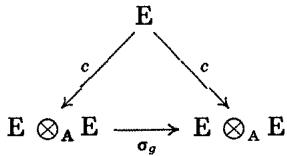
\includegraphics[keepaspectratio]{images/part004_b841500b.jpg}}

是交换的。

证明与第2号的命题2的证明类似。

当分次余代数 E 满足命题6的条件时，称其为余反交换的。

例。由第1号公式 (8) 直接可得，对每个 A-模 M，分次余代数 \(\bigwedge(M)\) 是余反交换的。

\subsection{双代数与斜双代数}

定义3. 环A上的分次双代数（相应地，斜分次双代数）是一个集合E，它带有N型的分次A-代数结构和N型的分次A-余代数结构，且两者具有相同的底层分次A-模结构，并满足：

\begin{enumerate}
\def\labelenumi{(\arabic{enumi})}
\item
  A-代数 E 是结合的且有单位元的。
\item
  A-余代数 E 是余结合的且有余单位。
\item
  余积 \(c: \mathbf{E} \to \mathbf{E} \otimes_{\mathbf{A}} \mathbf{E}\) 是从分次代数 \(\mathbf{E}\) 到分次代数 \(\mathbf{E} \otimes_{\mathbf{A}} \mathbf{E}\) （相应地，分次代数 \(\mathbf{E}^{\mathfrak{g}} \otimes_{\mathbf{A}} \mathbf{E}\) ，参见§4，第7号）中的同态。
\item
  余单位 \(\gamma\) （E 的）是从分次代数 E 到代数 A（带平凡分次）中的分次代数同态，使得若 e 表示 A-代数 \(\mathbf{E}, \gamma(e) = 1\) 。
\end{enumerate}

如果 E 是一个分次双代数且其分次是平凡的，则 E 简称为双代数。一个分次双代数称为交换的（相应地，余交换的），如果其底代数是交换的（相应地，如果其底余代数是余交换的）；一个斜分次双代数称为反交换的（相应地，余反交换的），如果其底分次代数是反交换的（相应地，如果其底分次余代数是余反交换的）。

由定义3及第2节命题5可知，对于分次双代数或斜分次双代数E，

\[
\left\{ \begin{array}{c} c (e) = e \otimes e \\ c (x) \equiv x \otimes e + e \otimes x (\mathrm{mod.} \mathrm{E} _ {+} \otimes \mathrm{E} _ {+}) \quad \text { for } x \in \mathrm{E} _ {+} = \bigoplus_ {n \geqslant 1} \mathrm{E} _ {n}. \end{array} \right.\tag{22}
\]

若E和F是两个分次双代数（相应地，两个斜分次双代数），则一个映射 \(\phi: \mathrm{E} \to \mathrm{F}\) 称为分次双代数态射（相应地，斜分次双代数态射），如果：（1） \(\phi\) 是一个分次代数态射（因此将E的单位元映到F的单位元）；（2） \(\phi\) 是一个分次余代数态射，使得若 \(\gamma\) 和 \(\gamma'\) 分别是E和F的余单位，则 \(\gamma = \gamma' \circ \phi\) .

例子。（1）设 S 是一个具有单位元 u 的幺半群，于是幺半群 S 在 A 上的代数 \(E = A^{(S)}\) 具有单位元 \(e_{u}\) (§2，第6号)；另一方面已经看到，E 典范地具有一个带余单位 \(\gamma\) 的余结合、余交换 A-余代数结构，使得 \(\gamma(e_{s}) = 1\) （对所有 \(s \in S\) ）（第1号，例4及第2号，例4、例5和例6）。给出余积的公式 \(c(e_{s}) = e_{s} \otimes e_{s}\) 也立即表明 c 是一个代数同态。因此在 E 上定义了一个余交换双代数结构，带此结构的 E 被称为幺半群 S 在 A 上的双代数。

如果 T 是另一个带有单位元的幺半群， \(v, f: \mathrm{S} \to \mathrm{T}\) 为一个同态，使得 \(f(u) = v\) ，而 \(f_{(\mathbf{A})}: \mathrm{A}^{(\mathrm{S})} \to \mathrm{A}^{(\mathrm{T})}\) 为由 \(f(\S 2, \text{no. } 6)\) 导出的 A-代数同态，则可立即验证 \(f_{(\mathbf{A})}\) 是一个双代数同态。

\begin{enumerate}
\def\labelenumi{(\arabic{enumi})}
\setcounter{enumi}{1}
\item
  设 M 为一个 A-模。在 S(M) 上定义的分次 A-代数（§ 6，第 1 号）和分次 A-余代数（第 1 号，例 6）结构，在此集合上定义了一个交换余交换的分次双代数结构；因为我们已经看到（第 1 号，例 6），S(M) 上的余积是一个代数同态，并且由余单位 \(\gamma\) 的定义（第2号，例6）可知 \(\gamma(1) = 1\) ，且 \(\gamma\) 是从 \(E\) 到 \(A\) 中的代数同态。
\item
  设 M 为 A-模。我们如同例 2 中那样看到， \(\bigwedge\) (M) 上的分次 A-代数（§ 7，第 1 号）和分次 A-余代数（第 1 号，例 7）结构在此集合上定义一个反交换、余反交换的斜分次双代数结构。
\end{enumerate}

注：若 M 是一个 A-模，使得 \(M \otimes_{A} M \neq \{0\}\) ，则分次 A-代数（§ 5，第 1 号）和分次 A-余代数（第 1 号，例 5）在 T(M) 上的结构并不定义一个双代数结构，因为一般地

\[
c (x _ {1} x _ {2} y _ {1} y _ {2}) \neq c (x _ {1} x _ {2}) c (y _ {1} y _ {2})
\]

对 M 的四个元素 \(x_{1}, x_{2}, y_{1}, y_{2}\) 成立，如第1号公式 (3) 所示。

\subsection{分次对偶 T(M)*gr、S(M)*gr 与 ∧(M)*gr}

从现在起，我们回到关于代数的章节的一般约定，因此（除非另有说明）假定这些代数是结合的且有单位的。

设 M 为一个 A-模；定义在 T(M)（第 1 号，例 5）、S(M)（第 1 号，例 6）和 \(\bigwedge\) (M)（第1号，例7）上的分次 A-余代数结构，依据第 2 号的命题 1 和命题 3 以及关于分次模的分次对偶的分次所作的约定（第 1 号），使我们能够典范地在分次对偶 T(M)*gr、S(M)*gr 和 \(\bigwedge\) (M)*gr 上定义 N 型分次代数结构。此外，分次代数 S(M)*gr 是交换的（第 2 号，命题 2 和例 5），且分次代数 \(\bigwedge\) (M)*gr 是反交换的（第3号，命题6及例）。在 \(\bigwedge\) (M)*gr 中，每个次数为 1 的元素的平方为零；这样的元素等同于 M 上的一个线性形式 \(f\) ，其平方是交错双线性形式 \(f \wedge f\) （在 M \(^{2}\) 上），使得

\[
(f \wedge f) (x, y) = f (x) f (y) - f (y) f (x)
\]

（第 2 号，例 3）。

设 \(\mathbf{N}\) 是另一个 A-模，且 \(u\) 为从 \(\mathbf{M}\) 到 \(\mathbf{N}\) 中的一个 A-线性映射。我们知道 \(u\) 典范地定义分次代数同态

\[
\left\{ \begin{array}{l} \mathsf {T} (u): \mathsf {T} (\mathbf {M}) \to \mathsf {T} (\mathbf {N}) \\ \mathsf {S} (u): \mathsf {S} (\mathbf {M}) \to \mathsf {S} (\mathbf {N}) \\ \bigwedge (u): \bigwedge (\mathbf {M}) \to \bigwedge (\mathbf {N}) \end{array} \right.\tag{23}
\]

（§ 5，第 2 号，§ 6，第 2 号和 § 7，第 2 号）。由第 1 号的公式 (3) 可立即验证 \(\mathsf{T}(u)\) 也是余代数态射。另一方面，若 \(\Delta_{\mathbf{M}}\) （相应地 \(\Delta_{\mathbf{N}}\) ）

表示对角映射 \(\mathbf{M} \to \mathbf{M} \times \mathbf{M}\) （相应地 \(\mathbf{N} \to \mathbf{N} \times \mathbf{N}\) ），则有关系式 \((u \times u) \circ \Delta_{\mathbf{M}} = \Delta_{\mathbf{N}} \circ u\) ；由此可得 \(\mathbf{S}(u \times u) \circ \mathbf{S}(\Delta_{\mathbf{M}}) = \mathbf{S}(\Delta_{\mathbf{N}}) \circ \mathbf{S}(u)\)

\[
(\text { resp. } \bigwedge (u \times u) \circ \bigwedge (\Delta_ {\mathbf {M}}) = \bigwedge (\Delta_ {\mathbf {N}}) \circ \bigwedge (u)).
\]

利用 \(\mathsf{S}(\mathbf{M})\) 和 \(\bigwedge (\mathbf{M})\) 中余积的定义（第 1 号，例 6 和 7）以及典范同构的函子性质，

\[
\mathbf {S} (\mathbf {M} \times \mathbf {M}) \rightarrow \mathbf {S} (\mathbf {M}) \otimes_ {\mathbf {A}} \mathbf {S} (\mathbf {M})
\]

和 \(\bigwedge (\mathbf{M}\times \mathbf{M})\to \bigwedge (\mathbf{M})^{\mathfrak{g}}\otimes_{\mathbf{A}}\bigwedge (\mathbf{M})\) ，可以看出 \(S(u)\) 和 \(\bigwedge (u)\) 也是余代数态射†（因此在这种情况下是双代数态射）。由此立即得出同态 (23) 的分次转置（II，§ 11，第 6 号）

\[
\begin{array}{c} ^ {t} \mathsf {T} (u): \mathsf {T} (\mathbf {N}) ^ {* \mathrm{gr}} \to \mathsf {T} (\mathbf {M}) ^ {* \mathrm{gr}} \\ ^ {t} \mathsf {S} (u): \mathsf {S} (\mathbf {N}) ^ {* \mathrm{gr}} \to \mathsf {S} (\mathbf {M}) ^ {* \mathrm{gr}} \\ ^ {t} \bigwedge (u): \bigwedge (\mathbf {N}) ^ {* \mathrm{gr}} \to \bigwedge (\mathbf {M}) ^ {* \mathrm{gr}} \end{array}
\]

是分次代数同态。

我们现在注意到，M 的对偶 M* 与 T(M)*gr（相应地，S(M)*gr，∧(M)*gr）中次数为 1 的元素所构成的子模等同。因此，由张量代数的泛性质（§ 5，第 1 号）和对称代数的泛性质（§ 6，第 1 号）可知，存在且仅存在一个分次代数同态

\[
\theta_ {\mathsf {T}}: T (M ^ {*}) \rightarrow T (M) ^ {* \mathrm{gr}}
\]

它延拓了典范单射 \(\mathbf{M}^{*}\to \mathsf{T}(\mathbf{M})^{*\mathrm{gr}}\) ，并且存在唯一一个分次代数同态

\[
\theta_ {\mathsf {S}}: S (M ^ {*}) \rightarrow S (M) ^ {* \mathrm{gr}}
\]

它延拓了典范单射 \(\mathbf{M}^{*}\to\mathsf{S}(\mathbf{M})^{*\mathrm{gr}}\) 。另一方面， \(\mathbf{M}^{*}\) 在 \(\bigwedge(\mathbf{M})^{*\mathrm{gr}}\) 的反代数中的典范单射使得 \(\mathbf{M}^{*}\) 的每个元素的平方为零；因此（§ 7，第 1 号，命题 1）存在唯一一个分次代数同态

\[
\theta_ {\wedge}: \bigwedge (\mathbf {M} ^ {*}) \rightarrow (\bigwedge (\mathbf {M}) ^ {* \mathrm{gr}}) ^ {\circ}
\]

它延拓了典范单射 \(M^{*}\to\bigwedge(M)^{*gr.}\) 。这些同态是函子性的：例如，对于每个 A-模同态 \(u:M\to N\) ，该图表

\pandocbounded{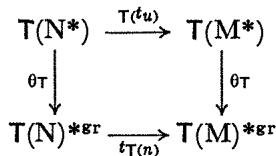
\includegraphics[keepaspectratio]{images/part004_1f4c9f33.jpg}}

是交换的，这直接从张量代数的泛性质（§ 5，第 1 号）得出；对 \(\theta_{s}\) 和 \(\theta_{\wedge}\) 也有类似的交换图。

我们将明确找出同态 \(\theta_{\mathsf{T}}\) , \(\theta_{\mathsf{S}}\) 和 \(\theta_{\wedge}\) 。为此，我们更一般地考虑一个带余积 \(c\) 的余结合 A-余代数 E，并对 \(n\) （ \(n \geqslant 2\) ）归纳地定义线性映射 \(c_{n}\) （从 E 到 \(\mathrm{E}^{\otimes n}\) 中），由 \(c_{2} = c\) 和

\[
c _ {n} = \left(c _ {n - 1} \otimes 1 _ {\mathrm{E}}\right) \circ c.\tag{24}
\]

另一方面，我们用 \(m_{n}:A^{\otimes n}\to A\) 表示典范线性映射，使得 \(m_{n}(\xi_{1}\otimes\xi_{2}\otimes\cdots\otimes\xi_{n})=\xi_{1}\xi_{2}\ldots\xi_{n}\) ，并注意，对 \(n\geqslant2\) ，

\[
m _ {n} = m \circ (m _ {n - 1} \otimes 1 _ {\mathbf {A}})\tag{25}
\]

记 \(m = m_2\) 。利用此记号：

引理1. (i) 在结合代数 \(\mathbf{E}^* = \operatorname{Hom}_{\mathbf{A}}(\mathbf{E}, \mathbf{A})\) 中， \(n\) 个 1 次元素 \(u_1, u_2, \ldots, u_n\) 的乘积由

\[
u _ {1} u _ {2} \dots u _ {n} = m _ {n} \circ (u _ {1} \otimes u _ {2} \otimes \dots \otimes u _ {n}) \circ c _ {n}.\tag{26}
\]

\begin{enumerate}
\def\labelenumi{(\roman{enumi})}
\setcounter{enumi}{1}
\tightlist
\item
  还假设余代数 E 是分次的。那么，在分次结合代数 \(\mathbf{E}^{*\mathrm{gr}} = \operatorname{Homgr}_{\mathbf{A}}(\mathbf{E}, \mathbf{A})\) 中， \(n\) 个 1 次元素 \(u_1, u_2, \ldots, u_n\) 的乘积由
\end{enumerate}

\[
u _ {1} u _ {2} \dots u _ {n} = m _ {n} \circ (u _ {1} \otimes u _ {2} \otimes \dots \otimes u _ {n}) \circ \delta_ {n}\tag{27}
\]

（其中 \(\delta_n: \mathbf{E} \to \mathbf{E}^{\otimes n}\) 是把每个 \(x \in \mathbf{E}\) 映为 \(c_n(x)\) 的多重次数 \((1, 1, \ldots, 1)\) 分量的线性映射。

公式（26）正是 \(\mathbf{E}^*\) 中乘积在 \(n = 2\) 时的定义；要对 \(n\) 用归纳法证明它，观察到

\[
\begin{array}{l} u _ {1} u _ {2} \dots u _ {n} \\ \qquad = m \circ ((u _ {1} u _ {2} \dots u _ {n - 1}) \otimes u _ {n}) \circ c \\ \qquad = m \circ ((m _ {n - 1} \circ (u _ {1} \otimes u _ {2} \otimes \dots \otimes u _ {n - 1}) \circ c _ {n - 1}) \otimes u _ {n}) \circ c \\ \qquad = m \circ (m _ {n - 1} \otimes \mathrm{l} _ {\mathrm{A}}) \circ (u _ {1} \otimes u _ {2} \otimes \dots \otimes u _ {n - 1} \otimes u _ {n}) \circ (c _ {n - 1} \otimes \mathrm{l} _ {\mathrm{E}}) \circ c \\ \qquad = m _ {n} \circ (u _ {1} \otimes u _ {2} \otimes \dots \otimes u _ {n}) \circ c _ {n} \end{array}
\]

根据（24）、（25）、II，§3，第3号，公式（5）以及关系式

\[
u _ {n} = 1 _ {\mathbf {A}} \circ u _ {n} \circ 1 _ {\mathbf {E}}.
\]

当 E 是分次的且元素 \(u_{i} \in E^{*gr}\) 是 1 次齐次的时，根据定义，对齐次元素 \(x_{i} \in E\) ，

\[
(u _ {1} \otimes u _ {2} \otimes \dots \otimes u _ {n}) (x _ {1} \otimes x _ {2} \otimes \dots \otimes x _ {n}) = 0
\]

除非所有 \(x_{i}\) 的次数均为 1，由此得到公式 (27) 。

由第1号中的公式 (3)、(5)和(7)以及公式 (24) 可知，当 E 取为三个分次余代数 \(\mathsf{T}(\mathbf{M})\) , \(\mathsf{S}(\mathbf{M})\) 和 \(\bigwedge (\mathbf{M})\) 之一时，对 \(n\) 用归纳法（利用余积是次数为 0 的分次同态这一事实）分别得到，对 M 中的 \(x_{1}, x_{2}, \ldots, x_{n}\) ：

\[
\text { when   } \mathrm{E} = \mathrm{T} (\mathrm{M}), \quad \delta_ {n} (x _ {1} x _ {2} \dots x _ {n}) = x _ {1} \otimes x _ {2} \otimes \dots \otimes x _ {n}
\]

\[
\text { when } \mathrm{E} = \mathrm{S(M)}, \quad \delta_ {n} (x _ {1} x _ {2} \dots x _ {n}) = \sum_ {\sigma \in \mathfrak {S} _ {n}} x _ {\sigma (1)} \otimes x _ {\sigma (2)} \otimes \dots \otimes x _ {\sigma (n)}
\]

\[
\text { when } \mathrm{E} = \bigwedge (\mathrm{M}), \quad \delta_ {n} (x _ {1} x _ {2} \dots x _ {n}) = \sum_ {\sigma \in \mathfrak {S} _ {n}} \varepsilon_ {\sigma}. x _ {\sigma (1)} \otimes x _ {\sigma (2)} \otimes \dots \otimes x _ {\sigma (n)}.
\]

只需注意，例如当 \(\mathbf{E} = \bigwedge (\mathbf{M})\) 时，在由第1号公式 (8) 得出的表达式 \(c_{n}(x_{1}x_{2}\ldots x_{n}) = (c_{n - 1}\otimes 1_{\mathbb{E}})\left(\sum (-1)^{\nu}(x_{i_1}\ldots x_{i_p})\otimes (x_{j_1}\ldots x_{j_{n - p}})\right)\) 中，唯一能给出多重次数 \((1,1,\dots ,1)\) 项的是那些使 \(n - p = 1\) 的项，因此

\[
\delta_ {n} (x _ {1} x _ {2} \dots x _ {n})
\]

是以下和中多重次数为 \((1, 1, \ldots, 1)\) 的项

\[
\sum_ {i = 1} ^ {n} (- 1) ^ {n - i} c _ {n - 1} \left(x _ {1} \dots x _ {i - 1} x _ {i + 1} \dots x _ {n}\right) \otimes x _ {i}
\]

且这一项必然等于

\[
\sum_ {i = 1} ^ {n} (- 1) ^ {n - i} \delta_ {n - 1} (x _ {1} \dots x _ {i - 1} x _ {i + 1} \dots x _ {n}) \otimes x _ {i},
\]

因此由归纳假设可得结果。

根据引理1， \(\mathsf{T}(\mathbf{M})^{*\mathrm{gr}}\) 中 \(n\) 个线性形式 \(x_{1}^{*}, x_{2}^{*}, \ldots, x_{n}^{*}\) （属于 \(\mathbf{M}^{*}\) ）的乘积由以下公式给出

\[
\left\langle x _ {1} ^ {*} x _ {2} ^ {*} \dots x _ {n} ^ {*}, x _ {1} x _ {2} \dots x _ {n} \right\rangle = \prod_ {i = 1} ^ {n} \left\langle x _ {i} ^ {*}, x _ {i} \right\rangle\tag{28}
\]

对 \(x_{i} \in \mathbf{M} (1 \leqslant i \leqslant n)\) 成立；这 \(n\) 个形式在 \(S(M)^{*gr}\) 中的乘积由以下公式给出

\[
\left\langle x _ {1} ^ {*} x _ {2} ^ {*} \dots x _ {n} ^ {*}, x _ {1} x _ {2} \dots x _ {n} \right\rangle = \sum_ {\sigma \in \mathfrak {S} _ {n}} \left(\prod_ {i = 1} ^ {n} \left\langle x _ {\sigma (i)} ^ {*}, x _ {i} \right\rangle\right);\tag{29}
\]

最后，这些形式在 \(\bigwedge (\mathbf{M})^{*\mathrm{gr}}\) 中的乘积由以下公式给出

\[
\langle x _ {1} ^ {*} x _ {2} ^ {*} \dots x _ {n} ^ {*}, x _ {1} x _ {2} \dots x _ {n} \rangle = \det (\langle x _ {i} ^ {*}, x _ {j} \rangle).\tag{30}
\]

在三种情形中，我们分别有

\[
\theta_ {T} (x _ {1} ^ {*} \otimes x _ {2} ^ {*} \otimes \dots \otimes x _ {n} ^ {*}) = x _ {1} ^ {*} x _ {2} ^ {*} \dots x _ {n} ^ {*}
\]

\[
\theta_ {S} (x _ {1} ^ {*} x _ {2} ^ {*} \dots x _ {n} ^ {*}) = x _ {1} ^ {*} x _ {2} ^ {*} \dots x _ {n} ^ {*}
\]

\[
\theta_ {\wedge} (x _ {1} ^ {*} \wedge x _ {2} ^ {*} \wedge \dots \wedge x _ {n} ^ {*}) = x _ {n} ^ {*} x _ {n - 1} ^ {*} \dots x _ {1} ^ {*} = (- 1) ^ {n (n - 1) / 2} x _ {1} ^ {*} x _ {2} ^ {*} \dots x _ {n} ^ {*}
\]

因此，我们从 (28)、(29) 和 (30) 推导出以下关系式

\[
\langle \theta_ {T} (x _ {1} ^ {*} \otimes x _ {2} ^ {*} \otimes \dots \otimes x _ {n} ^ {*}), x _ {1} \otimes x _ {2} \otimes \dots \otimes x _ {n} \rangle = \prod_ {i = 1} ^ {n} \langle x _ {i} ^ {*}, x _ {i} \rangle\tag{28 bis}
\]

（换言之， \(\theta_{\mathsf{T}}\) 在 \(\mathsf{T}^2 (\mathbf{M}^*)\) 上的限制就是 II，§4，第4号中的典范同态）

\[
\langle \theta_ {\mathsf {S}} (x _ {1} ^ {*} x _ {2} ^ {*} \dots x _ {n} ^ {*}), x _ {1} x _ {2} \dots x _ {n} \rangle = \sum_ {\sigma \in \mathfrak {S} _ {n}} \left(\prod_ {i = 1} ^ {n} \langle x _ {\sigma (i)} ^ {*}, x _ {i} \rangle\right)\tag{29 bis}
\]

\[
\begin{array}{r l} (30 \text { bis}) &\langle \theta_ {\wedge} (x _ {1} ^ {*} \wedge x _ {2} ^ {*} \wedge \dots \wedge x _ {n} ^ {*}), x _ {1} \wedge x _ {2} \wedge \dots \wedge x _ {n} \rangle \\ & \qquad = (- 1) ^ {n (n - 1) / 2} \mathrm{det} (\langle x _ {i} ^ {*}, x _ {j} \rangle). \end{array}
\]

命题7. 设 \(\mathbf{M}\) 是有限生成的投射 A-模。则典范同态 \(\theta_{\mathsf{T}}: \mathsf{T}(\mathbf{M}^{*}) \to \mathsf{T}(\mathbf{M})^{*\mathrm{gr}}\) 和 \(\theta_{\wedge}: \bigwedge (\mathbf{M}^{*}) \to (\bigwedge (\mathbf{M})^{*\mathrm{gr}})^{0}\) 是双射。此外，分次对偶 \(\bigwedge (\mathbf{M})^{*\mathrm{gr}}\) 此时等于对偶 \(\bigwedge (\mathbf{M})^{*}\) ，即 A-模 \(\bigwedge (\mathbf{M})\) 的对偶。

首先假设 \(\mathbf{M}\) 具有有限基 \((e_i)_{1\leq i\leq m}\) ，并设 \((e_i^*)_{1\leq i\leq m}\) 为 \(\mathbf{M}^*\) 的对偶基 (II, § 10, no. 4)。公式 (28 bis) 表明，对每个有限序列 \(s = (j_k)_{1\leq k\leq n}\) （ \(n\) 个元素取自区间 \([1,m]\) （ \(\mathbf{N}\) 的）），

\[
\theta_ {\mathsf {T}} (e _ {j _ {1}} ^ {*} \otimes \dots \otimes e _ {j _ {n}} ^ {*})
\]

是指标为 \(s\) 的元素，位于 \((\mathsf{T}^n (\mathbf{M}))^*\) 的基中，该基对偶于 \(\mathsf{T}^n (\mathbf{M})\) 的由 \(e_s = e_{j_1}\otimes \dots \otimes e_{j_n}\) 组成的基（§ 5，第 5 号，定理 1）。因此 \(\theta_{\mathsf{T}}\) 是双射。

类似地，公式（30 bis）表明，对每个有限子集 \(\mathbf{H}\) （属于 \([1, m]\) ，含 \(n\) 个元素）， \((-1)^{n(n-1)/2} \theta_{\wedge}(e_{\mathrm{H}}^{*})\) （§7，第8号，定理1的记号）是指标为 \(\mathbf{H}\) 的元素，位于 \((\bigwedge^{n}(\mathbf{M}))^{*}\) 的基中，该基对偶于 \(\bigwedge^{n}(\mathbf{M})\) 的由 \(e_{\mathrm{H}}\) 组成的基。因此 \(\theta_{\wedge}\) 是双射。

现在仅假设 M 是有限生成且投射的；则 M 是有限生成自由 A-模 L 的一个直和因子，因此存在两个

A-线性映射 \(M \xrightarrow{j} L \xrightarrow{p} M\) ，其复合为恒等映射 \(1_{M}\) 。由此我们推导出一个交换图

\pandocbounded{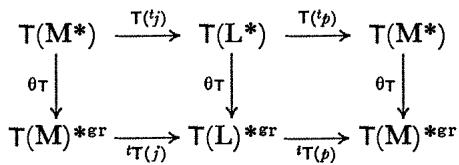
\includegraphics[keepaspectratio]{images/part004_2d3cbe02.jpg}}

以及一个类似的交换图，其中 \(\mathsf{T}\) 被替换为 \(\bigwedge\) 。该命题随后由以下引理得出：

引理2. 设

\pandocbounded{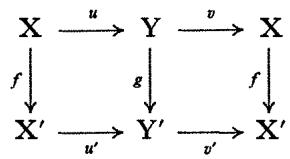
\includegraphics[keepaspectratio]{images/part004_a09507a7.jpg}}

是一个集合与映射的交换图，使得 \(v \circ u\) 和 \(v' \circ u'\) 分别是 \(X\) 和 \(X'\) 的恒等映射。那么，若 \(g\) 是单射（相应地，满射、双射），则 \(f\) 亦然。

u 是单射，因为 \(v \circ u\) 是；因此，若 g 是单射， \(u' \circ f = g \circ u\) 是单射，从而 f 是单射。类似地 \(v'\) 是满射，因为 \(v' \circ u'\) 是；因此，若 g 是满射， \(f \circ v = v' \circ g\) 是满射，从而 f 是满射。

命题7的最后断言由以下事实得出： \(\bigwedge (\mathbf{M})\) 此时是一个有限生成的 A-模（§ 7，第 3 号，命题 6 及 II，§ 11，第 6 号，注记）。

我们现在考察关于同态 \(\theta_{\mathsf{S}}\) （当 \(\mathbf{M}\) 是投射的且有限生成时）可以说些什么。首先假设 \(\mathbf{M}\) 具有有限基 \((e_i)_{1\leq i\leq m}\) 。在本章开头的记号中，A-模 \(\mathbf{S}^n (\mathbf{M})\) 以元素族 \(e^{\alpha}\) （满足 \(|\alpha | = n\) ）为基。设 \(u_{\alpha}\) （对于 \(|\alpha | = n\) ）表示指标为 \(\alpha\) 的元素，位于 \((\mathbf{S}^n (\mathbf{M}))^*\) 的对偶于 \((e^{\alpha})\) 的基中。元素 \(u_{\alpha}\) （对于 \(\alpha \in \mathbf{N}^m\) ）因此构成代数 \(\mathbf{S}(\mathbf{M})^{*\mathrm{gr}}\) 的基，我们将显式给出这个基的乘法表。我们记

\[
u _ {\alpha} u _ {\beta} = \sum_ {\gamma \in \mathbf {N} ^ {m}} a _ {\alpha \beta \gamma} u _ {\gamma} \quad \text { with } a _ {\alpha \beta \gamma} \in \mathrm{A}.
\]

那么根据定义

\[
a _ {\alpha \beta \gamma} = \langle u _ {\alpha} u _ {\beta}, e ^ {\gamma} \rangle = m ((u _ {\alpha} \otimes u _ {\beta}) (c (e ^ {\gamma}))),
\]

（其中 \(m: \mathbf{A} \otimes \mathbf{A} \to \mathbf{A}\) 定义 \(\mathbf{A}\) 上的乘法， \(c\) 是 \(\mathsf{S}(\mathbf{M})\) 的余积。换言之， \(a_{\alpha \beta \gamma}\) 正是 \(e^{\alpha} \otimes e^{\beta}\) 的系数（当 \(c(e^{\gamma})\) 用 \(\mathsf{S}(\mathbf{M})\otimes \mathsf{S}(\mathbf{M})\) 的由 \(e^{\xi}\otimes e^{\eta}\) 组成的基表示时），其中 \(\xi\) 和 \(\eta\) 遍历 \(\mathbf{N}^m\) 。但由于 \(c\) 是代数同态，

\[
c (e ^ {\gamma}) = \prod_ {i = 1} ^ {m} (c (e _ {i})) ^ {\gamma_ {i}} = \prod_ {i = 1} ^ {m} (e _ {i} \otimes 1 + 1 \otimes e _ {i}) ^ {\gamma_ {i}}
\]

根据第1号公式 (4)，这给出

\[
c (e ^ {\gamma}) = \sum_ {\xi + \eta = \gamma} (\xi , \eta) e ^ {\xi} \otimes e ^ {\eta}\tag{31}
\]

其中我们记

\[
((\xi , \eta)) = \prod_ {i = 1} ^ {n} \frac {(\xi_ {i} + \eta_ {i}) !}{\xi_ {i} ! \eta_ {i} !} \quad (\text { cf.   } \S 10, \text {   no.   } 4, \text {   formula   (18) }).\tag{32}
\]

因此我们得到乘法表

\[
u _ {\alpha} u _ {\beta} = ((\alpha , \beta)) u _ {\alpha + \beta}.\tag{33}
\]

另一方面，如果 \((e_i^*)_{1\leq i\leq m}\) 是 \(\mathbf{M}^*\) 的、对偶于 \((e_i)\) 的基，则由公式 (29 bis) 可知，对所有 \(\alpha \in \mathbf{N}^m\) ，

\[
\theta_ {S} (e ^ {* \alpha}) = \alpha ! u _ {\alpha}\tag{34}
\]

在 §6 第6号的记号中。因此同态 \(\theta_{\mathsf{S}}\) 是双射当且仅当诸 \(\alpha!u_{\alpha}\) 构成 \(\mathsf{S}(\mathbf{M})^{*\mathrm{gr}}\) 的一组基，亦即诸元素 \(\alpha!1\) 均可逆。

命题8. 假设环 A 是有理数域 Q 上的代数；那么，对于每个有限生成的投射 A-模 M，同态

\[
\theta_ {\mathsf {S}}: S (M ^ {*}) \rightarrow S (M) ^ {* \mathrm{gr}}
\]

是双射。

这相当于在M有限生成且自由的情形下证明；我们像命题7的证明中那样，利用引理2从这一情形过渡到一般情形。

注记。设 M 为一个 A-模，且 \(\rho: \mathbf{A} \to \mathbf{B}\) 为一个交换环同态。则存在一个分次 B-代数同态的交换图

\[
\begin{array}{l} \mathsf {T} ((\mathbf {M} ^ {*}) _ {(B)}) \longrightarrow (\mathsf {T} (\mathbf {M}) ^ {* \mathrm{gr}}) _ {(B)} \\ \mathsf {T} (\upsilon_ {\mathbf {M}}) \Biggl \downarrow \qquad \qquad \qquad \qquad \qquad \qquad \qquad \qquad \qquad \Biggl \downarrow \upsilon_ {\mathbf {T} (\mathbf {M})} \\ \mathsf {T} ((\mathbf {M} _ {(B)}) ^ {*}) \xrightarrow [ \theta_ {\mathsf {T}} ]{} \mathsf {T} (\mathbf {M} _ {(B)}) ^ {* \mathrm{gr}} \end{array}
\]

其中第一行是由同态 \(\theta_{\mathsf{T}}\otimes 1_{\mathsf{B}}\colon \mathsf{T}(\mathbf{M}^{*})\otimes_{\mathbf{A}}\mathbf{B}\to \mathsf{T}(\mathbf{M})^{*\mathrm{gr}}\) 与典范同构

\[
\mathsf {T} ((\mathbf {M} ^ {*}) _ {(\mathbf {B})}) \rightarrow \mathsf {T} (\mathbf {M} ^ {*}) \otimes_ {\mathbf {A}} \mathbf {B}
\]

（§ 5，第 3 号，命题 5）复合而成的同态。利用公式 (28) 及同态 \(\upsilon_{\mathbf{E}}\) （II，§ 5，第 4 号）的定义，可立即验证此图表是交换的。当 \(\mathbf{M}\) 是有限生成的投射 A-模时， \(\mathbf{M}_{(\mathbf{B})}\) 是有限生成的投射 B-模（II，§ 5，第 1 号，命题 4 的推论），且上述图表中的所有同态都是双射（命题 7 及 II，§ 5，第 4 号，命题 8）。存在类似的交换图，其中 \(\mathsf{T}\) 被替换为 \(\mathsf{S}\) 或 \(\bigwedge\) ；关于 \(\bigwedge\) 的那个图当 \(\mathbf{M}\) 是投射的且有限生成时也由双射同态组成（命题 7）；若进一步 \(\mathbf{A}\) 是 \(\mathbf{Q}\) 上的代数，则关于 \(\mathsf{S}\) 的图也由双射同态组成（命题 8）。

\subsection{内乘：代数情形}

设 \(E = \bigoplus_{p \geqslant 0} E_p\) 是一个 N 型分次 A-代数，P 是一个 Z 型分次 A-模；对每个齐次元素 \(x \in E_p\) ，用 \(x\) 左乘是 E 到自身的 A-线性映射 \(e(x)\) ，它是 \(p\) 次分次映射。对每个元素 \(u \in \text{Homgr}_A(E, P)\) ， \(u\) 被 \(x\) 的右内乘记作 \(u \llcorner x\) ，它就是元素 \(u \circ e(x)\) （属于 \(\text{Homgr}_A(E, P)\) ）。我们还记 \((i(x))(u) = u \llcorner x\) ，于是可见 \(i(x)\) 是 \(p\) 次分次自同态（分次 A-模 \(\text{Homgr}_A(E, P)\) 的）。若现在 \(x = \sum_{p \geqslant 0} x_p\) 是 E 的任意元素（其中 \(x_p \in E_p\) （对一切 \(p \geqslant 0\) ），且 \(x_p = 0\) （除 \(p\) 的有限个值外）），我们记 \(i(x) = \sum_{p=0}^{\infty} i(x_p)\) ，它因此是 A-模 \(\text{Homgr}_A(E, P)\) 的自同态。

为了记住在表达式 \(u \llcorner x\) 中哪个元素“作用”于另一个元素，注意“作用”于 u 的元素 x 位于 \(\llcorner\) 中水平线的自由端。

代数 E 的结合性转化为关系 \(e(xy) = e(x) \circ e(y)\) （对齐次的 x, y）；因此，根据 \(i(x)\) 的定义，

\[
i (x y) = i (y) \circ i (x)\tag{35}
\]

首先对齐次的 \(x, y\) ，然后通过线性性，对 E 中任意的 \(x, y\) ；这也可以写成

\[
(u \llcorner x) \llcorner y = u \llcorner (x y)\tag{36}
\]

对于 \(x, y\) （在 \(\mathbf{E}\) 中）及 \(u \in \operatorname{Homgr}_{\mathbf{A}}(\mathbf{E}, \mathbf{P})\) ；另一方面，显然 \(i(1)\) 是恒等映射（因为由 \(e(1) = 1_{\mathbf{E}}\) 即得），且 \(x \mapsto i(x)\) 是 A-线性的，于是可以看出，外合成律 \((x, u) \mapsto u \llcorner x\) （ \(x \in \mathbf{E}\) ， \(u \in \operatorname{Homgr}_{\mathbf{A}}(\mathbf{E}, \mathbf{P})\) ）与加法一起，在 \(\operatorname{Homgr}_{\mathbf{A}}(\mathbf{E}, \mathbf{P})\) 上定义了一个右 E-模结构。

特别地，我们考虑 P = A 的情形， \(\operatorname{Homgr}_{\mathbf{A}}(\mathbf{E}, \mathbf{P})\) 在此情形下是 E 的分次对偶 \(E^{*gr}\) ； \(i(x)\) 则是 A-线性映射 \(e(x)\) 的分次转置（II，§11，第6号），换言之，对 E 中所有 x, y 及 \(u \in E^{*gr}\) ，

\[
\langle u \llcorner x, y \rangle = \langle u, x y \rangle .\tag{37}
\]

按照本段开头的约定，注意，若 \(x \in E_{p}\) ，则 \(i(x)\) 是 \(E^{*gr}\) 的 -p 次自同态。

对每个齐次元素 \(x \in \mathbf{E}_p\) ，用 \(x\) 右乘类似地记作 \(e'(x)\) ，而元素 \(u \circ e'(x)\) （属于 \(\operatorname{Homgr}_{\mathbf{A}}(\mathbf{E}, \mathbf{P})\) ）称为 \(u\) 被 \(x\) 的左内乘，记作 \(x \lrcorner u\) ；我们记 \(i'(x) = x \lrcorner u\) ，于是 \(i'(x)\) 是 \(\operatorname{Homgr}_{\mathbf{A}}(\mathbf{E}, \mathbf{P})\) 的 \(p\) 次分次自同态；如上所述，此定义可推广到 \(x\) 是 \(\mathbf{E}\) 的任意元素的情形。由于这时 \(e'(xy) = e'(y)e'(x)\) ，

\[
i ^ {\prime} (x y) = i ^ {\prime} (x) \circ i ^ {\prime} (y)\tag{38}
\]

也可以写作

\[
x \lrcorner (y \lrcorner u) = (x y) \lrcorner u\tag{39}
\]

并且表明外合成律 \((x,u)\mapsto x\lrcorner u\) 与加法一起，在 \(\operatorname{Homgr}_{\mathbf{A}}(\operatorname{E},\operatorname{P})\) 上定义了一个左 E-模结构。另一方面，E 的结合性蕴含 \(e(x)\circ e'(y)=e'(y)\circ e(x)\) （对 E 中齐次的 x,y），由此得到关系式

\[
(y \lrcorner u) \llcorner x = y \lrcorner (u \llcorner x)\tag{40}
\]

从而使 \(\mathrm{Homgr}_{\mathbf{A}}(\mathbf{E},\mathbf{P})\) 上的两个外合成律在此集合上定义一个 (E, E)-双模结构（II，§ 1，第14号）。

当我们取 \(\mathbf{P} = \mathbf{A}\) 时， \(i'(x)\) 是 \(e'(x)\) 的分次转置；换言之，对所有 \(x, y\) （在 \(\mathbf{E}\) 中）及 \(u \in \mathbf{E}^{*\mathrm{gr}}\) ，

\[
\langle y, x \lrcorner u \rangle = \langle y x, u \rangle .\tag{41}
\]

当分次代数 E 是交换的时，显然 \(u \llcorner x = x \lrcorner u\) 。当 E 是反交换的且 P = A 时，则对于 \(x \in E_{p}\) 、 \(y \in E_{r}\) 和 \(u \in E_{q}^{*}\) ，有 \(yx = (-1)^{pr}xy\) ，由此，由 (37) 和 (41) 得 \(\langle u \llcorner x, y \rangle = (-1)^{pr}\langle y, x \lrcorner u \rangle\) 。但由于该关系的两边除 r = q - p 外均为零，

\[
x \lrcorner u = (- 1) ^ {p (q - p)} u \llcorner x.
\]

设 F 为另一个分次 A-代数，且 \(\phi: E \to F\) 为分次代数的一个 A-同态；则 \(\tilde{\phi} = \operatorname{Hom}(\phi, 1_{P}): \operatorname{Homgr}_{A}(F, P) \to \operatorname{Homgr}_{A}(E, P)\) 是 0 次的分次 A-同态；根据定义，对于 E 中的 \(x, y\) 及 \(u \in \operatorname{Homgr}_{A}(F, P)\) ，

\[
\begin{array}{r l} (\tilde {\phi} (u \llcorner \phi (x))) (y) & = (u \llcorner \phi (x)) (\phi (y)) \\ & = u (\phi (x) \phi (y)) = u (\phi (x y)) = (\tilde {\phi} (u)) (x y) = (\tilde {\phi} (u) \llcorner x) (y) \end{array}
\]

或等价地

\[
\tilde {\phi} (u \llcorner \phi (x)) = \tilde {\phi} (u) \llcorner x\tag{42}
\]

并且类似地

\[
\tilde {\phi} (\phi (x) \lrcorner u) = x \lrcorner \tilde {\phi} (u).\tag{43}
\]

换句话说，当 \(\operatorname{Homgr}_{\mathbf{A}}(\mathbf{F}, \mathbf{P})\) 借助环同态 \(\phi: \mathbf{E} \to \mathbf{F}\) 被视为 (E, E)-双模时，可以看出 \(\tilde{\phi}\) 是一个 (E, E)-双模同态（或者是把 (F, F)-双模 \(\operatorname{Homgr}_{\mathbf{A}}(\mathbf{F}, \mathbf{P})\) 映入 (E, E)-双模 \(\operatorname{Homgr}_{\mathbf{A}}(\mathbf{E}, \mathbf{P})\) 的 E-同态）。

例子。特别地，当 E 是分次代数 \(\mathsf{T}(\mathbf{M})\) 、 \(\mathsf{S}(\mathbf{M})\) 或 \(\bigwedge(\mathbf{M})\) 之一（其中 M 是一个 A-模），而 P 是一个 A-模（带有平凡分次）时，上述内容可以应用。为了显式求出如此得到的双模结构，注意 \(\operatorname{Homgr}_{\mathbf{A}}(\mathsf{T}(\mathbf{M}),\mathbf{P})\) （相应地 \(\operatorname{Homgr}_{\mathbf{A}}(\mathsf{S}(\mathbf{M}),\mathbf{P})\) 、 \(\operatorname{Homgr}_{\mathbf{A}}(\bigwedge(\mathbf{M}),\mathbf{P})\) ）中 -n 次的元素与从 \(M^{n}\) 到 P 的 n 重线性映射（相应地，对称 n 重线性映射、交错 n 重线性映射）等同。只需表出乘积

\[
f \llcorner (x _ {1} \otimes x _ {2} \otimes \dots \otimes x _ {p})
\]

\((\text{resp. } f \llcorner (x_1 x_2 \ldots x_p), \text{ resp. } f \llcorner (x_1 \wedge x_2 \wedge \dots \wedge x_p))\) （对 M 中元素的每个有限序列 \((x_i)_{1 \leq i \leq p}\) ）以及左内乘的类似表达式。由定义立即得出

\[
f \llcorner (x _ {1} \otimes x _ {2} \otimes \dots \otimes x _ {p}) = (x _ {1} \otimes x _ {2} \otimes \dots \otimes x _ {p}) \lrcorner f = 0\tag{44}
\]

若 \(p > n\) ，并且对于 \(p \leqslant n, f \llcorner (x_1 \otimes x_2 \otimes \dots \otimes x_p)\) （相应地

\[
\left(x _ {1} \otimes x _ {2} \otimes \dots \otimes x _ {p}\right) \lrcorner f)
\]

是由下式定义的 \((n - p)\) -线性映射：

\[
\left\{ \begin{array}{l} (f \llcorner (x _ {1} \otimes x _ {2} \otimes \dots \otimes x _ {p})) (y _ {1}, \ldots , y _ {n - p}) \\ = f (x _ {1}, \ldots , x _ {p}, y _ {1}, \ldots , y _ {n - p}) \\ ((x _ {1} \otimes x _ {2} \otimes \dots \otimes x _ {p}) \lrcorner f) (y _ {1}, \ldots , y _ {n - p}) \\ = f (y _ {1}, \ldots , y _ {n - p}, x _ {1}, \ldots , x _ {p}). \end{array} \right.\tag{45}
\]

对于 \(p > n\) ，在 \(\operatorname{Homgr}_{\mathbf{A}}(\mathsf{S}(\mathbf{M}), \mathbf{P})\) （相应地 \(\operatorname{Homgr}_{\mathbf{A}}(\bigwedge(\mathbf{M}), \mathbf{P})\) ）中也有公式 (44)，其中 \(x_1 \otimes x_2 \otimes \cdots \otimes x_p\) 替换为 \(x_1x_2 \ldots x_p\) （相应地 \(x_1 \wedge x_2 \wedge \cdots \wedge x_p\) ）。对于 \(p \leqslant n\) ，在 (45) 中进行相同的替换，就定义了对称 \((n - p)\) -线性映射 \(f \llcorner (x_1x_2 \ldots x_p)\) 和 \((x_1x_2 \ldots x_p) \lrcorner f\) （相应地，交错 \((n - p)\) -线性映射

\[
f \llcorner (x _ {1} \wedge x _ {2} \wedge \dots \wedge x _ {p}) \quad \text { and } \quad (x _ {1} \wedge x _ {2} \wedge \dots \wedge x _ {p}) \lrcorner f).
\]

当 \(n = p\) 时，上述乘积等于 \(\mathbf{M}\) 上等于 \(f(x_{1},\ldots ,x_{p})\) 的常值函数。

若 \(u: \mathbf{M} \to \mathbf{N}\) 是 A-模同态，则 \(\mathsf{T}(u): \mathsf{T}(\mathbf{M}) \to \mathsf{T}(\mathbf{N})\) 是分次 A-代数同态，于是由我们上面所见可知， \((\mathsf{T}(u))^{\sim}\) 是 \(\mathsf{T}(\mathbf{M})\) -同态，把 \((\mathsf{T}(\mathbf{N}), \mathsf{T}(\mathbf{N}))\) -双模 \(\operatorname{Homgr}_{\mathbf{A}}(\mathsf{T}(\mathbf{N}), \mathbf{P})\) 映入 \((\mathsf{T}(\mathbf{M}), \mathsf{T}(\mathbf{M}))\) -双模 \(\operatorname{Homgr}_{\mathbf{A}}(\mathsf{T}(\mathbf{M}), \mathbf{P})\) ，相对于环同态 \(\mathsf{T}(u)\) 。对 \((\mathbf{S}(u))^{\sim}\) 和 \((\bigwedge(u))^{\sim}\) 有类似的结果。
